\documentclass[9pt,twocolumn]{extarticle}
\usepackage[margin=1.5cm,columnsep=0.6cm]{geometry}
\usepackage{graphicx}
\usepackage{amsmath,amssymb}
\usepackage{amsthm}
\usepackage{placeins}
\usepackage{enumitem}
\newtheorem{proposition}{Proposition}
\newtheorem{corollary}{Corollary}
\usepackage{booktabs}
\usepackage{multirow}
\usepackage{hyperref}
\usepackage{xcolor}
\usepackage{caption}
\usepackage{times}
\hypersetup{colorlinks=true,linkcolor=blue,citecolor=blue,urlcolor=blue}
\captionsetup{font=footnotesize,labelfont=bf}

\title{\vspace{-1.2cm}\textbf{QEM, QEC, or FTQC? An Empirical Decision Layer for\\
Quantum Circuit Reduction Techniques, Validated Against the State of the Art}}
\author{\footnotesize Independent research project \\[-2pt]
\footnotesize \texttt{alberto.maldo1312@gmail.com}}
\date{\footnotesize September 26, 2026}

\begin{document}
\maketitle

\begin{abstract}
\noindent
Choosing whether a quantum circuit should run under quantum error mitigation
(QEM), quantum error correction (QEC), or full fault-tolerant quantum
computing (FTQC) depends critically on which circuit-reduction technique is
applied beforehand --- a dependency rarely made explicit in practice. This
work builds and empirically validates a decision layer
(\texttt{technique\_advisor}/\texttt{decide\_regime}) that profiles a circuit,
recommends which of seven reduction techniques to try, and chooses between
QEM and FTQC under a hard qubit-budget constraint, using real backend
calibration data throughout. All techniques are measured on a common,
basis-gate-normalized footing to avoid a class of measurement error
(artificially collapsed T-count) that we document and correct. Across a
98-instance, 9-family circuit dataset we find that spectral sparsification of
the circuit's interaction graph is a reasonable single predictor of whether
ZX-calculus reduction helps, but --- on rigorous re-verification with
leave-one-family-out (LOFO) cross-validation on the complete dataset --- its
honest accuracy is $70.4\%$, statistically indistinguishable from a trivial
majority-class baseline, correcting an earlier, non-held-out figure of
$82.9\%$ that we retract here. We further report: (i) a real, from-scratch
simulation of a rotated surface code (Stim + PyMatching) whose measured
threshold ($\sim\!0.5$--$0.8\%$) is consistent with the published value
($\sim\!1\%$, Fowler et al. 2012) and which we connect to our FTQC
resource-estimation pipeline, fixing a real bug in the process (a measured
physical error rate that was computed but never passed to the estimator),
and later refit per noise model with Deltakit, which lowers the
superconducting (SI1000) threshold to $0.40\%$ --- enough that at $0.32\%$ no
surface-code distance helps our flagship circuit, which needs
$p_{2q}\lesssim0.25\%$ first;
(ii) that optimized QAOA at depth $p=1,2,3$ never outperforms simple
classical simulated annealing on any of 27 tested MaxCut instances; and
(iii) that tensor-network contraction cost, tested as an alternative
classical-simulability proxy, does not correlate with spectral
sparsifiability ($r=0.16$) but shows a suggestive, unvalidated correlation
with ZX-calculus gain ($r=0.66$, $n=9$). QAOA-type circuits remain the one
structural case that no tested predictor --- statistical or otherwise ---
classifies reliably, and we report this as an open limitation rather than
a solved problem.
\end{abstract}

\section{Introduction}
Whether a given quantum algorithm should run under QEM (mitigation, no
logical qubits), QEC (correction with moderate overhead), or full FTQC (large
overhead, arbitrarily low error) is usually treated as a fixed property of
the available hardware. We show instead that it is a function of the circuit
\emph{after} a reduction technique has been applied --- and that the choice
of technique can flip the decision. Motivated by this, we cumulatively
evaluated nine circuit-reduction and analysis techniques, always requiring
(a) a real backend basis-gate set for T-count/2-qubit-count measurement, (b)
comparison against published numbers wherever available, and (c) honest
reporting of negative results. This paper consolidates a full research
session into a single, reproducible account: what each technique measurably
does, where a proposed decision layer works, where it does not, and where a
previously reported number had to be corrected after a cleaner
re-verification.

\paragraph{Contributions, and the theory each one draws on.} Every
technique below is measured empirically in this paper (section numbers are
where it is used), but is grounded --- explicitly, not by association --- in
a specific piece of prior theory, or declared as our own heuristic when it
is not:
\begin{itemize}[leftmargin=*,itemsep=1pt,topsep=2pt]
\item \textbf{ZX-calculus T-count reduction} (\S\ref{sec:results}):
phase-polynomial normal-form rewriting~\cite{kissinger2019}.
\item \textbf{RZZ gate teleportation}: Clifford+T optimization via matroid
partitioning~\cite{amy2014}.
\item \textbf{AND-gate measurement-based uncomputation}: ancilla reuse via
mid-circuit measurement; a heuristic of this project, with no external
theorem behind it.
\item \textbf{Bounded QCP tracking with an RQAOA-style extension}: the
symmetry-protection obstruction theory behind RQAOA~\cite{bravyi2020},
combined with the independently-developed BQCP tracker
(\texttt{github.com/1nnocenzo/bqcp}).
\item \textbf{Circuit cutting}: wire-cutting / quasi-probability
decomposition, as implemented in \texttt{qiskit-addon-cutting}~\cite{qiskitcutting}.
\item \textbf{RQAOA correlation reproduction}: \cite{bravyi2020}.
\item \textbf{SwapStrategy vs.\ SabreSwap routing}: both are Qiskit's own
heuristic transpiler passes; no external theorem is under test here, only
a direct empirical comparison.
\item \textbf{Rotated surface code} (\S\ref{sec:qec}): the surface-code
threshold theorem~\cite{fowler2012}, decoded with real minimum-weight
perfect matching.
\item \textbf{Tensor-network contraction cost} (\S\ref{sec:tensor}): the
standard classical-hardness metric from the quantum-advantage
literature~\cite{boixo2018}, related to treewidth-based simulation
cost~\cite{markovshi2008}.
\item \textbf{QAOA as Ising ground-state search} (\S\ref{sec:qaoa-ising}):
the original QAOA formulation~\cite{farhi2014}.
\item \textbf{Spectral sparsifiability predictor}: graph sparsification by
effective resistance~\cite{spielman2011}.
\item \textbf{FTQC resource estimation}: the Azure Quantum Resource
Estimator~\cite{azureqre}, and, for our own independent estimator, the
Litinski lattice-surgery magic-state factory cost
model~\cite{litinski2019game}.
\item \textbf{Entanglement / classical-simulability metric}
(\S\ref{sec:entanglement-metric}): entanglement-entropy diagnostics from
tensor-network simulation of real hardware~\cite{tindall2023tensor},
alongside the treewidth bound~\cite{markovshi2008}.
\item \textbf{Dynamic circuits / iterative phase estimation}
(\S\ref{sec:iqpe}): the semiclassical, iterative QFT~\cite{griffithsniu1996}.
\item \textbf{External validation}: IBM's quantum-utility
experiment~\cite{kim2023utility}, used as an independent benchmark this
project did not design.
\item \textbf{Propositions~1--3} (\S\ref{sec:new-theory}): phase-polynomial
theory~\cite{kissinger2019} plus elementary Boolean Fourier /
Walsh--Hadamard character independence (Prop.~1); the Markov~\&~Shi
treewidth-simulation theorem~\cite{markovshi2008} (Prop.~2); and a direct
algebraic consequence of this project's own calibrated surface-code fit
and the Litinski factory-cost formula~\cite{litinski2019game} (Prop.~3).
\item \textbf{Stress test: scale, learned predictors, operational cost}
(\S\ref{sec:stresstest}): standard supervised learning
(\texttt{scikit-learn} logistic regression and decision trees) with
\texttt{LeaveOneGroupOut} cross-validation, applied honestly to this
project's own features rather than to a new theory.
\end{itemize}

\section{Tools and instrumentation}
\label{sec:tools}
Every result in this paper comes from a real library call, not a hand
estimate. Table~\ref{tab:tools} lists, per technique, the exact tool used to
produce its numbers, so any figure below can be traced back to the code that
generated it.

\begin{table}[t]
\centering\footnotesize
\caption{Tooling used to produce every measured result in this paper.}
\label{tab:tools}
\begin{tabular}{@{}p{2.1cm}p{5.6cm}@{}}
\toprule
Technique / result & Tool(s) \\
\midrule
Basis normalization & Qiskit \texttt{transpile()} to \texttt{FakeTorino}'s
\texttt{cz, rz, sx, x} basis \\
ZX-calculus & \texttt{pyzx.full\_reduce()} (real T-count reduction) \\
Unitary-equivalence check & \texttt{qiskit.quantum\_info.Operator} \\
RZZ gate teleportation & Qiskit \texttt{QuantumCircuit} construction + real
basis-count \\
AND-gate uncomputation & Custom heuristic over Qiskit DAG (\texttt{qiskit.
converters.circuit\_to\_dag}) \\
Bounded QCP + RQAOA rounds & Custom tracker, cross-checked vs.\ BQCP
(\texttt{github.com/1nnocenzo/bqcp}) \\
Circuit cutting & \texttt{qiskit-addon-cutting} (\texttt{find\_cuts},
\texttt{partition\_problem}) \\
RQAOA correlation & Qiskit \texttt{Statevector} exact expectation values \\
Routing & Qiskit \texttt{SwapStrategy} and \texttt{SabreSwap} passes \\
Spectral sparsifiability & \texttt{networkx} (Laplacian, effective
resistance via pseudo-inverse) \\
Tensor-network cost & \texttt{cotengra} (\texttt{HyperOptimizer}),
\texttt{opt\_einsum}, \texttt{quimb}, \texttt{kahypar} \\
QAOA ground state & Exact brute force (\texttt{numpy}), classical simulated
annealing (custom), QAOA optimization via \texttt{scipy.optimize} (Nelder--Mead)
over exact \texttt{Statevector} expectation \\
Real QEC (surface code) & \texttt{stim} (syndrome circuit generation \&
sampling), \texttt{pymatching} (MWPM decoding) \\
FTQC resource estimates & Azure Quantum Resource Estimator (QRE), called
with a custom \texttt{qubitParams} profile built from the real measured
\texttt{p\_phys} \\
QEM cost model & Real 2-qubit error rate from a \texttt{FakeTorino}-transpiled
circuit (\texttt{qiskit\_aer.noise}) \\
\bottomrule
\end{tabular}
\end{table}

\section{Methodology}
\textbf{Basis-gate normalization.} All circuits are transpiled to a fixed
real basis (\texttt{cz, rz, sx, x}, matching IBM's \texttt{FakeTorino}) before
any T-count or 2-qubit-count measurement. Skipping this step lets a
transpiler silently absorb non-Clifford rotations into Clifford gates,
producing an artificially collapsed (often zero) T-count --- a bug we
encountered and fixed early in this project and continued to guard against
throughout.

\textbf{Honest generalization testing.} Every accuracy figure in this paper
is \emph{leave-one-family-out} (LOFO): a classifier is trained on all
circuit families except one, then tested only on the held-out family. We
adopt this after finding that ordinary random $k$-fold cross-validation
inflates apparent accuracy by leaking information between near-identical
variants of the same family (e.g. \texttt{QFT\_n5}/\texttt{QFT\_n6}); LOFO is
the only test in this paper that measures generalization to a genuinely
unseen circuit structure.

\textbf{Verify before trusting a good result.} Twice during this project a
result that looked like a genuine discovery was rejected after a rigorous
check: (1) a from-scratch GF(2) phase-polynomial fusion algebra appeared to
out-perform \texttt{pyzx.full\_reduce()}, until an explicit unitary
equivalence check (via \texttt{qiskit.quantum\_info.Operator}) showed the
``optimized'' circuit was not unitarily equivalent to the original (maximum
operator difference $1.35$, far beyond a global phase) --- so this
reimplementation was discarded and \texttt{full\_reduce()} is used directly
throughout; (2) a headline $82.9\%$ LOFO accuracy for a proposed predictor
did not reproduce under a clean re-run on the complete dataset (Section
\ref{sec:decision-layer}), and is retracted here in favor of the correct,
verified figure.

\section{Circuit dataset}
The dataset used for the decision-layer and predictor experiments (Sections
\ref{sec:decision-layer}--\ref{sec:qec}) contains 98 circuits across 9
structurally distinct families, built with real Qiskit library components:
QFT ($n=3$--$12$), Cuccaro ripple-carry adders ($n=2$--$8$ bits), QAOA-style
cost+mixer circuits on random graphs ($n=6$--$16$, edge density
$0.2$--$0.8$), unstructured random circuits, GHZ state preparation,
\texttt{TwoLocal} VQE ans\"atze, Grover's operator with a diagonal oracle,
Toffoli chains, and quantum phase estimation. Ground truth for ``does
ZX-calculus help'' is $\ge 10\%$ real T-count reduction from
\texttt{full\_reduce()}, measured on the basis-normalized circuit.

\section{Individual technique results}
\label{sec:results}

\subsection{ZX-calculus T-count reduction}
Real gain from \texttt{pyzx.full\_reduce()}, basis-normalized, averaged per
family: QPE $77.5\%$, QFT $45.3\%$, Cuccaro adder $42.9\%$ (constant across
sizes), Toffoli chain $21.7\%$, VQE ansatz $21.0\%$, Grover $18.4\%$, random
circuits $15.3\%$, GHZ $0.0\%$ (trivial, no T-gates), and \textbf{QAOA
$0.0\%$ in all 24 tested instances, without exception}. This is explained by
the published, deterministic phase-gadget fusion criterion (Kissinger \&
van~de~Wetering, arXiv:1903.10477): two phase gadgets fuse only if they act
on exactly the same qubit support, a condition QAOA's independent
edge-local $ZZ$ rotations typically violate while QFT/adder/Toffoli-chain's
repeated, overlapping structure satisfies.

\subsection{Cheap pre-check vs.\ full reduction}
We compared a cheap, non-restructuring pass
(\texttt{interior\_clifford\_simp}+\texttt{gadget\_simp}, gadget fusion only
on already-aligned gadgets) against full \texttt{full\_reduce()} (which adds
pivoting-based restructuring) across the 91 non-trivial circuits. The cheap
check predicts the full result within 5 percentage points in $57.1\%$ of
cases and is only $1.7\times$ faster on average --- the pivoting step
contributes a non-trivial share of the total gain (e.g.\ Toffoli chains:
cheap check reports $0\%$ vs.\ a real $14$--$26\%$), so the cheap pre-check is
not a reliable stand-in for the full reduction.

\subsection{RZZ gate teleportation}
Helps when the interaction graph's average degree is below $\sim15$ (25/27
tested instances improved); the one real negative case found
(\texttt{MANN-a9}) has average degree $\sim40$.

\subsection{AND-gate measurement-based uncomputation}
Requires genuine ancilla candidates (qubits whose last use precedes the
circuit's midpoint); a declared, honest limitation is that this heuristic
cannot automatically verify the ancilla is discarded to $|0\rangle$ rather than
reused, as in the Cuccaro adder.

\subsection{Bounded QCP tracking and an RQAOA-style extension}
We extend bounded quantum constant-propagation tracking (validated against
BQCP, \texttt{github.com/1nnocenzo/bqcp}) with an RQAOA-inspired rule:
instead of abandoning tracking once a group exceeds the qubit budget
$n_{pcm}$, we fix the most-confident qubit (largest $|P(0)-P(1)|$, the direct
analogue of RQAOA's largest $|\langle Z_iZ_j\rangle|$) and count the number
of such fixing rounds needed. Sanity-checked on independent GHZ-3 blocks
(exactly 3 rounds, fidelity loss $\approx 0.5$/round, when the budget forces
fixing). On real circuits ($n_{pcm}=4,6,8$): the Cuccaro adder and QAOA need
the most rounds (20--33), dropping sharply for QFT/random circuits as the
budget grows. This metric is exploratory and has no external benchmark to
compare against yet.

\subsection{Circuit cutting}
Using the real \texttt{qiskit-addon-cutting} \texttt{find\_cuts} solver: the
Cuccaro adder (chain-like, highly separable) needs 2 cuts / $256\times$
sampling overhead; a dense QAOA instance needs 18--46 cuts /
$10^{17}$--$10^{44}\times$ overhead depending on subcircuit-size constraints
--- intractable in practice. The true driver is structural separability
(minimum cut size of the interaction graph), not qubit count.

\subsection{RQAOA correlation reproduction}
We reproduce $\langle Z_iZ_j\rangle$ directly via Qiskit statevector
(\texttt{openqaoa-core} is no longer installable under Python $\ge 3.11$) and
find $r=-0.95$ between interaction-graph degree and correlation strength ---
the \emph{opposite} sign of our original hypothesis, reported as measured.

\subsection{SwapStrategy vs.\ SabreSwap routing}
\texttt{SwapStrategy} produces a constant $\sim120$ SWAPs across a graph
density sweep ($0.15$--$1.00$); SabreSwap ranges from 18 to 274 SWAPs and then
\emph{drops} to 132 at density $1.0$ --- a real, twice-reproduced anomaly
(independent random graph instances) that remains unexplained. Two real
SWAP-counting bugs (forced \texttt{basis\_gates} and \texttt{decompose(reps
$\ge$ 1)} both silently synthesize SWAP$\to$3$\times$CX before counting) were
found and fixed to obtain these numbers.

\subsection{Real quantum error correction: a rotated surface code}
\label{sec:qec}
All FTQC cost figures elsewhere in this paper come from the Azure Quantum
Resource Estimator (QRE), an analytical resource model. To obtain an
independent, first-principles data point, we built a genuine QEC experiment:
a rotated surface-code syndrome circuit generated with \texttt{Stim}
(\texttt{stim.Circuit.generated}, exact Clifford-circuit simulation, not an
approximation) decoded with real minimum-weight perfect matching
(\texttt{PyMatching}), sweeping code distance $d\in\{3,5,7\}$ and physical
error rate $p\in[0.001,0.10]$ with $20{,}000$ shots per point
(Fig.~\ref{fig:qec}). The measured threshold ($p^\ast\approx 0.5$--$0.8\%$,
the point above which increasing $d$ stops helping) is consistent, in order
of magnitude, with the published surface-code threshold ($\sim1\%$ under
depolarizing noise; Fowler et al.\ 2012). We then connected this simulation
to the resource-estimation pipeline as a cross-check
(\texttt{cross\_validate\_logical\_error\_rate}), which in the process
surfaced and fixed a real bug: the function that calls Azure QRE accepted a
measured physical error rate \texttt{p\_phys} but never passed it into the
solver, always using a fixed generic qubit profile regardless of the actual
hardware measured. The cross-check itself is honestly limited: at $5{,}000$
shots, statistical resolution cannot confirm logical error rates as low as
Azure QRE's analytical prediction (e.g.\ $3\times10^{-7}$); both figures are
reported together with their uncertainty rather than treated as confirmed
agreement.

\begin{figure}[t]
\centering
\includegraphics[width=\linewidth]{figs/qec_threshold_plot.png}
\caption{Measured logical error rate vs.\ physical error rate for a rotated
surface code (Stim + PyMatching, 20{,}000 shots/point). The threshold
crossover between $d=3$ and $d=7$ falls between $p=0.005$ and $p=0.008$.}
\label{fig:qec}
\end{figure}

\subsection{Tensor-network contraction cost as a classical-simulability proxy}
\label{sec:tensor}
We tested whether classical simulability, measured as the cost of
contracting the circuit's tensor network for a single transition amplitude
(the standard hardness metric from the quantum-advantage literature, e.g.\
Boixo et al.\ 2018), is a useful structural feature. Each circuit is
represented as a real index network (one tensor per gate after basis
normalization) and \texttt{cotengra.HyperOptimizer} --- whose default search
uses simulated annealing to minimize contraction cost, the same class of
combinatorial optimization used in Section~\ref{sec:qaoa-ising} --- finds a
contraction order. On one representative instance per family
(Fig.~\ref{fig:tensor}), the resulting contraction width does \emph{not}
correlate with spectral sparsifiability ($r=0.16$, essentially null): these
are genuinely different structural properties, contradicting our initial
hypothesis that they would be interchangeable. It does show a moderate
correlation with real ZX-calculus gain ($r=0.66$), which is suggestive but
based on only 9 points (one per family) and has not been tested with LOFO.

\begin{figure}[t]
\centering
\includegraphics[width=\linewidth]{figs/tensor_network_correlation.png}
\caption{Tensor-network contraction cost vs.\ spectral sparsifiability
(left, $r=0.16$) and vs.\ real ZX-calculus gain (right, $r=0.66$), one
instance per family.}
\label{fig:tensor}
\end{figure}

\subsection{QAOA as an Ising ground-state problem}
\label{sec:qaoa-ising}
QAOA circuits in our dataset encode a MaxCut/Ising problem on a random
graph. We solved the same 24 problem instances three ways: exact brute force
($2^n$ enumeration, $n\le16$), classical simulated annealing (single-spin
flips, temperature schedule, no quantum component), and QAOA at $p=1$ with
genuinely optimized parameters (Nelder-Mead over the exact statevector
expectation value, several random restarts). \textbf{Simulated annealing
matches the exact optimum in 24/24 instances; optimized QAOA $p=1$ reaches
an average approximation ratio of $0.740$ and never beats classical
annealing in any instance.} Extending to $p=2,3$ on a smaller 9-instance
subset (Fig.~\ref{fig:qaoa-depth}), the ratio improves only slightly
($0.708\to0.738$ on average) and \textbf{never crosses $1.0$ in any of the 27
tested instances at any depth} --- consistent with, and not contradicting,
the well-documented result that shallow QAOA rarely beats a good classical
heuristic on small random graphs. The fixed, unoptimized parameters
originally used to build this project's QAOA dataset ($\gamma=0.7,
\beta=0.4$) perform worse still, an additional honest caveat about the
dataset's QAOA instances.

\begin{figure}[t]
\centering
\includegraphics[width=\linewidth]{figs/qaoa_depth_sweep.png}
\caption{QAOA approximation ratio at $p=1,2,3$ vs.\ the classical
simulated-annealing baseline (always $=1.0$). No instance at any depth
closes the gap.}
\label{fig:qaoa-depth}
\end{figure}

\section{The decision layer}
\label{sec:decision-layer}

\subsection{Architecture}
\texttt{technique\_advisor.py} profiles a circuit (interaction-graph degree,
T-count fraction, ancilla candidates, bounded-QCP knowable fraction,
spectral sparsifiability) and recommends each of the seven techniques above.
\texttt{pipeline\_v2.py}/\texttt{decide\_regime()} compares real QEM
expected time-to-reliable-answer (shot time $\times\,1/\text{fidelity}^2$,
using real 2-qubit error rates from a transpiled circuit on
\texttt{FakeTorino}) against Azure QRE's FTQC runtime and physical-qubit
estimate, applying a hard qubit-budget feasibility cut before ZX-calculus is
even attempted --- avoiding the false economy of reducing a circuit that
could never fit the available hardware regardless.

\subsection{A retracted number, and what replaced it}
An earlier iteration of this project reported spectral sparsifiability of
the interaction graph (via effective resistance and the Laplacian
pseudo-inverse, Spielman--Srivastava) as an $82.9\%$-accurate LOFO predictor
of ZX-calculus benefit. On a clean re-implementation and a full re-run over
the complete 98-instance dataset with the identical LOFO protocol, this
figure did not reproduce: the correct value is \textbf{$70.4\%$}. Critically,
this is \emph{identical} to a trivial majority-class baseline (``assume
ZX-calculus helps by default, except when the T-count fraction is exactly
zero''). Table~\ref{tab:predictors} reports every predictor tested with the
same protocol; none exceeds this trivial baseline.

\begin{table}[t]
\centering\footnotesize
\caption{LOFO accuracy of every ZX-calculus-benefit predictor tested, on the
complete 98-instance dataset with an identical protocol.}
\label{tab:predictors}
\begin{tabular}{@{}lc@{}}
\toprule
Method & LOFO accuracy \\
\midrule
Majority-class baseline & $70.4\%$ \\
Fixed threshold (T-count frac.\ $>10\%$) & $70.4\%$ \\
Logistic regression: spectral sparsifiability & $70.4\%$ \\
Depth-2 tree: T-count frac.\ + max.\ degree & $49.0\%$ \\
Logistic regression: T-count frac.\ + max.\ degree & $59.2\%$ \\
Tensor-contraction cost alone (Sec.~\ref{sec:tensor}) & $59.2\%$ \\
Best 3-feature tree found & $67.3\%$ \\
\bottomrule
\end{tabular}
\end{table}

\subsection{Deployed rule and its honest confidence}
Given Table~\ref{tab:predictors}, the rule deployed in
\texttt{technique\_advisor.py} is: (i) if the T-count fraction is exactly
zero, recommend against ZX-calculus (an exact, deterministic filter, always
correct by construction); (ii) if the circuit shows the QAOA-like signature
(high maximum interaction-graph degree combined with moderate-to-high
spectral sparsifiability), emit a \textbf{low-confidence warning} rather
than a binary classification, since this is the one case where every tested
method fails (0/24 QAOA instances benefit, against every method's
prediction); (iii) otherwise, recommend ZX-calculus by default,
transparently reporting that this default is not backed by any feature that
outperforms it. This is a deliberate choice to report an honest $70.4\%$
confidence rather than a false, higher one.

\subsection{Chaining techniques}
We prototyped chaining circuit cutting into the decision layer
(\texttt{pipeline\_chain.py}): check real cutting feasibility
(\texttt{find\_cuts} sampling overhead against a declared budget of
$10^6$); if feasible, partition into real subcircuits
(\texttt{partition\_problem}) and run \texttt{technique\_advisor} on each
fragment separately. Verified on real circuits: a dense QAOA instance is
correctly rejected (overhead $7.9\times10^{43}\gg10^6$, falls back to
whole-circuit analysis); another instance partitions into three real
fragments (9, 7, and 1 qubits) that are each profiled independently. A
declared limitation: the automatic partitioner does not always split a
circuit further even when \texttt{find\_cuts} reports multiple cuts (as with
the Cuccaro adder in our tests), a genuine integration limitation, not a bug
we chose to hide.

\section{Benchmarking: technique $\times$ family $\times$ metric}
\label{sec:benchmarking}
This section collects, in one place, every technique's measured result
against every circuit family it was tested on, in the spirit of an open
community benchmark (Unitary Foundation's Metriq) but populated with this
project's own executed experiments rather than community submissions.

\subsection{Coverage heatmap}
Figure~\ref{fig:heatmap} shows which technique was measured on which circuit
family, and with what outcome (helps / does not help / warning), across the
full 98-instance, 9-family dataset. ZX-calculus is the only technique
measured across all 9 families; the other six were measured on a smaller set
of 4 reference circuits (QFT10, an 8-bit Cuccaro adder, a dense QAOA
instance, and an 8-qubit random circuit) and have not yet been extended to
the full dataset --- a scope limitation we state explicitly rather than
implying broader coverage than what was actually run.

\begin{figure}[t]
\centering
\includegraphics[width=\linewidth]{figs/technique_family_heatmap.png}
\caption{Coverage and outcome of every technique across circuit families:
green = measured benefit, red = measured no-benefit, yellow = warning /
depends on structure, gray = not yet measured on that family.}
\label{fig:heatmap}
\end{figure}

\subsection{ZX-calculus gain by family (full coverage)}
Table~\ref{tab:zxfamily} restates the per-family averages from
Section~\ref{sec:results} in benchmark form, since ZX-calculus is the one
technique with full 9-family coverage.

\begin{table}[t]
\centering\footnotesize
\caption{ZX-calculus T-count reduction by family, full 98-instance dataset.}
\label{tab:zxfamily}
\begin{tabular}{@{}lccc@{}}
\toprule
Family & $n$ & Mean gain & Range \\
\midrule
QPE & 5 & $77.5\%$ & $60.0$--$90.5\%$ \\
QFT & 10 & $45.3\%$ & $22.2$--$55.6\%$ \\
Adder (Cuccaro) & 7 & $42.9\%$ & constant \\
Toffoli chain & 7 & $21.7\%$ & $14.3$--$25.7\%$ \\
VQE ansatz & 12 & $21.0\%$ & $15.8$--$25.2\%$ \\
Grover & 5 & $18.4\%$ & $0.0$--$38.5\%$ \\
Random & 21 & $15.3\%$ & $7.4$--$22.3\%$ \\
GHZ & 7 & $0.0\%$ & constant (no T-gates) \\
\textbf{QAOA} & 24 & $\mathbf{0.0\%}$ & \textbf{constant, all 24} \\
\bottomrule
\end{tabular}
\end{table}

\subsection{Other six techniques: 4-reference-circuit spot check}
Table~\ref{tab:othertech} reports the remaining six techniques, measured
only on the 4 reference circuits described above --- the coverage this
project has today, not a claim of full-dataset validation.

\begin{table}[t]
\centering\footnotesize
\caption{Six additional techniques on 4 reference circuits (QFT10, Adder8,
QAOA/dense, Random8). ``Not yet'' = not extended to more families.}
\label{tab:othertech}
\begin{tabular}{@{}p{2.3cm}p{5.3cm}@{}}
\toprule
Technique & Outcome across the 4 references \\
\midrule
RZZ teleportation & Helps at low avg.\ degree (QFT10, Adder8, Random8);
depends on structure for dense QAOA \\
AND-gate uncompute & No clear ancilla candidates on QFT10/QAOA/Random8;
Adder8 has real candidates but needs manual reuse verification \\
Bounded QCP ($n_{pcm}{=}4$) & Partially trackable on QFT10/Adder8/Random8;
globally entangled (0\% trackable) on QAOA \\
Circuit cutting & Adder8: 2 cuts / $256\times$ overhead (feasible); QAOA:
18--46 cuts / $10^{17}$--$10^{44}\times$ overhead (infeasible) \\
RQAOA correlation & $r=-0.95$ on QAOA/dense (opposite sign of initial
hypothesis); not applicable to the other 3 families \\
RQAOA-style rounds & 20--33 rounds across QFT10/Adder8/QAOA/Random8 at
$n_{pcm}=4$--$8$, decreasing as budget grows \\
\bottomrule
\end{tabular}
\end{table}

\subsection{Routing benchmark: SWAP count and depth vs.\ graph density}
Figure~\ref{fig:density} shows the full density sweep behind the SwapStrategy
vs.\ SabreSwap comparison of Section~\ref{sec:results}.

\begin{figure}[t]
\centering
\includegraphics[width=\linewidth]{figs/fig1_density_sweep.pdf}
\caption{SWAP count (a) and circuit depth (b) vs.\ interaction-graph
density, for \texttt{SwapStrategy} (constant $\sim$120 SWAPs) and
\texttt{SabreSwap} (18 to 274 SWAPs, with an unexplained drop to 132 at
density $=1.0$).}
\label{fig:density}
\end{figure}

\subsection{Measured metrics vs.\ published ranges}
Figure~\ref{fig:lit} places every measured metric in this paper's scope
against the range reported in the corresponding published source (where one
exists), making explicit which of our numbers fall inside, at the edge of,
or (for the QAOA and predictor-accuracy results) outside the range the
literature would suggest.

\begin{figure}[t]
\centering
\includegraphics[width=\linewidth]{figs/fig2_technique_vs_literature.pdf}
\caption{This project's measured metrics vs.\ published reference ranges,
by technique.}
\label{fig:lit}
\end{figure}

\subsection{QEM vs.\ FTQC decision case study}
Figure~\ref{fig:regime} shows the actual quantity \texttt{decide\_regime()}
compares --- expected QEM time vs.\ FTQC (Azure QRE) runtime, in log scale,
before and after ZX-calculus reduction --- across four circuit families,
illustrating that reduction can shift which regime a circuit falls into.

\begin{figure}[t]
\centering
\includegraphics[width=\linewidth]{figs/fig3_regime_case.pdf}
\caption{Expected QEM vs.\ FTQC time, before and after ZX-calculus, for 4
circuit families (log scale). Reduction can move a circuit across the
QEM/FTQC decision boundary.}
\label{fig:regime}
\end{figure}

\subsection{BQCP comparison}
Figure~\ref{fig:bqcp} compares our static-circuit gate-count reduction under
bounded QCP tracking against BQCP's own reported reduction on its native
dynamic-circuit benchmarks --- a like-for-like external validation point for
one of the less-established techniques in Table~\ref{tab:othertech}.

\begin{figure}[t]
\centering
\includegraphics[width=\linewidth]{figs/fig4_bqcp.pdf}
\caption{Gate-count reduction from bounded QCP tracking: this project's
static circuits (red) vs.\ BQCP's own dynamic-circuit benchmarks (blue).}
\label{fig:bqcp}
\end{figure}

\subsection{RQAOA correlation}
Figure~\ref{fig:rqaoa} shows the measured relationship behind the
$r=-0.95$ figure reported in Section~\ref{sec:results}: correlation strength
$|\langle Z_iZ_j\rangle|$ against edge degree sum, on the dense QAOA
reference circuit.

\begin{figure}[t]
\centering
\includegraphics[width=\linewidth]{figs/fig5_rqaoa_correlation.pdf}
\caption{$|\langle Z_iZ_j\rangle|$ vs.\ edge degree sum on QAOA/dense
($r=-0.95$), the opposite sign from our original hypothesis.}
\label{fig:rqaoa}
\end{figure}

\subsection{Classical baselines for QAOA}
Figure~\ref{fig:qaoa-gs} shows the full density/size sweep behind the
Section~\ref{sec:qaoa-ising} result: optimized QAOA $p=1$ approximation
ratio against the classical simulated-annealing baseline (always at the
exact optimum, ratio $=1.0$), across all 24 tested graph instances.

\begin{figure}[t]
\centering
\includegraphics[width=\linewidth]{figs/qaoa_vs_classical_ground_state.png}
\caption{QAOA $p=1$ approximation ratio vs.\ classical simulated annealing
(exact optimum, ratio $=1.0$ in all 24 instances), by graph size and
density.}
\label{fig:qaoa-gs}
\end{figure}

\section{At what point does FTQC become applicable?}
\label{sec:crossover}
Section~\ref{sec:decision-layer} establishes a decision layer that compares
QEM and FTQC for a given circuit, but the four reference circuits used
throughout this paper (T-count 56--135) never favor FTQC, at any physical
error rate or qubit budget tested. That is a real, verified result (Section
\ref{sec:tools-open-estimator} below), but it does not by itself answer the
more useful question: at what point --- of hardware quality, qubit budget,
or problem size --- does FTQC start to win?

\subsection{An independent, self-derived FTQC resource estimator}
\label{sec:tools-open-estimator}
To answer this without depending solely on Azure QRE's semi-closed
analytical model, we built a second, fully independent and inspectable
estimator (\texttt{open\_resource\_estimator.py}). It uses the same
published functional form of the surface-code threshold (Fowler et al.
2012, $p_L(d) = A \cdot (p/p_{th})^{(d+1)/2}$), but with $A$ and $p_{th}$
fit directly to our own 27-point Stim+PyMatching dataset rather than taken
from any paper or vendor. An initial fit over all 27 points gave a poor
$R^2=0.28$; inspecting the residuals showed why: at $p_{\rm phys}\ge2\%$,
the logical error rate saturates near $0.5$ for every tested distance (the
``coin-flip'' regime, outside the power-law model's domain). Restricting
the fit to the 15 sub-threshold points ($p_{\rm phys}\le1\%$), weighted by
each point's own binomial standard error, gives $p_{th}=0.740\%\pm0.009$pp,
$A=0.0348$, $R^2=0.964$ --- a genuinely self-derived threshold, distinct
from both the visually-inspected crossover reported in Section
\ref{sec:qec} and the $\sim1\%$ literature value.

\paragraph{Revision: one threshold per noise model, measured with Deltakit.}
The fit above was measured on Stim's generated memory circuits, whose noise
model adds no error to qubits that sit idle during a layer of two-qubit
gates and gives measurement the same error rate as a gate. That is not the
noise of any real device, and it turns out to matter more than any other
assumption in this paper. We therefore refitted the model per circuit-level
noise model with Riverlane's open-source Deltakit (v0.10.2): its own
rotated-planar-code Z-memory experiments ($d$ rounds), decoded with
PyMatching, on $d\in\{3,\dots,11\}$ and a grid of $p$ below threshold, up to
$2\times10^6$ shots per point (\texttt{research/qec/fit\_threshold\_deltakit.py}).
The fit uses $d\geq5$ and $p\leq0.8\,p_{th}$ (refined iteratively), where the
power-law form is meant to hold:
\begin{center}
\begin{tabular}{llrrr}
\toprule
noise model & used for & $A$ & $p_{th}$ & $\chi^2$/dof \\
\midrule
SI1000 (2q $p$, 1q/idle $p/10$, meas.\ $5p$) & superconducting & 0.0589 & $0.404\%\pm0.005$ & 2.37 \\
ToyNoise (2q $p$, 1q/idle $p/10$, meas.\ $p$) & trapped ion & 0.0421 & $0.847\%\pm0.014$ & 2.13 \\
SD6 (every op.\ and idle $p$, native CX) & generic default & 0.0680 & $0.653\%\pm0.012$ & 5.61 \\
\bottomrule
\end{tabular}
\end{center}
Three checks (\texttt{examples/deltakit\_crosscheck.py}): (i) the original
$0.740\%$ is reproduced through Deltakit's decoding path on Stim's circuits
($0.720\%\pm0.012$), so the change is a noise-model change, not a tooling
artefact --- the gap to SD6 is the idle noise; (ii) on ten held-out points
not used in any fit, including $d=13$ beyond the fitted range, measured
$p_L$ stays within a factor $1.34$ of the prediction (the model is slightly
conservative at $d=13$); (iii) a bare rotated patch uses $2d^2-1$ physical
qubits, so we now count $2d^2$ per logical qubit (Litinski's tile, routing
included) instead of the $2d^2+3d-1$ read from Stim's \texttt{num\_qubits},
which counts unused qubit indices. Every hardware profile now carries its
noise model: SI1000 for the superconducting profile ($p=p_{2q}$), ToyNoise
for the trapped-ion profiles --- a declared approximation (cheap idles,
measurement comparable to a gate), not an ion-specific error model. All
estimates from here on use these fits.

Cross-validating this estimator against Azure QRE on the four reference
circuits shows runtime agreement within $1.1$--$2.1\times$, but a physical-qubit
count $24$--$46\times$ lower than Azure's. This large, consistent gap has an
identified cause, stated rather than hidden: our estimator does not model
magic-state distillation factories, which Azure QRE does include and which
dominate physical qubit count for T-gate-heavy algorithms. Consequently our
open estimator is used only as an order-of-magnitude runtime check; qubit
feasibility decisions still rely on Azure QRE throughout this paper.

\subsection{The crossover sweep}
Using the four real reference circuits as archetypes (their measured
qubit count, T-count, and two-qubit-gate count), we scaled each by
$1\times,10\times,100\times,1000\times$ (same circuit type at a larger
problem size, e.g.\ a bigger QFT or adder instance) and swept physical
error rate ($10^{-3}$ to $10^{-6}$) and available physical qubit budget
($10^3$ to $10^6$), using Azure QRE for FTQC feasibility/runtime and this
project's own validated QEM time model
($\text{shot\_time}\times1/\text{fidelity}^2$) for comparison.

\begin{figure}[t]
\centering
\includegraphics[width=\linewidth]{figs/ftqc_crossover_heatmap.png}
\caption{Where FTQC becomes applicable, physical error rate fixed at
today's measured value ($0.1\%$): infeasible (red), feasible but no clear
advantage (yellow), clear FTQC advantage $>10\times$ (green), by circuit
archetype, problem scale, and qubit budget.}
\label{fig:crossover}
\end{figure}

\textbf{Main finding, and a counter-intuitive one}: a clear FTQC advantage
(feasible and $>10\times$ faster than QEM) appears consistently once T-count
reaches roughly $1{,}000$--$15{,}000$, and in every archetype tested, this
crossover is already reached at \emph{today's} measured physical error rate
($p_{\rm phys}\le0.1\%$) --- not at some hypothetical future hardware
improvement. What is missing at that point is qubit budget alone (typically
$75{,}000$--$260{,}000$ physical qubits). We verified the opposite corner
explicitly: at the scale of our actual reference circuits, even with
$p_{\rm phys}=10^{-6}$ and a $1{,}000{,}000$-qubit budget, FTQC is feasible
but $8\times$ \emph{slower} than QEM for QFT10 ($1.74\times10^{-4}$s FTQC
vs.\ $2.08\times10^{-5}$s QEM) --- FTQC's fixed per-round overhead simply
does not amortize on a circuit this small, regardless of hardware quality.

The practical implication: at the gate quality already measured on real
hardware in this project, the binding constraint for reaching FTQC
advantage is qubit-count scale-up, not further error-rate improvement, once
an algorithm instance is large enough. This is a more specific and
actionable claim than ``it depends on the hardware,'' and it reframes what
this project's decision layer should report: not a single QEM-vs-FTQC
verdict, but the T-count crossover point and the qubit budget required at
that point, stated separately.

\subsection{A new lever, found by testing a larger real circuit: layout and routing search}
\label{sec:layout-search}
We extended testing beyond the four small reference circuits to a
16-qubit, T-count-3930 Shor-like circuit (recovered from an earlier stage
of this project) and to real VQE-ansatz and Grover circuits built from
Qiskit's circuit library. The two small circuits (VQE, T-count 48; Grover,
T-count 172) behave exactly like the four original references --- no FTQC
advantage at any tested hardware quality or qubit budget. The larger
circuit, whose T-count falls inside the crossover band identified above,
surfaced a genuinely new finding.

Transpiling it to \texttt{FakeTorino} with a single fixed configuration
(the pipeline's original approach: optimization level 1, one transpiler
seed) gave a measured physical error rate of $0.517\%$ --- close to our
original fitted surface-code threshold ($0.740\%$, Section~\ref{sec:tools-open-estimator};
under the SI1000 fit adopted later in that section, $0.517\%$ is already above threshold),
where required code distance (and thus physical qubit count) blows up
sharply. Azure QRE's resulting estimate: \textbf{4{,}425{,}210} physical
qubits. Inspecting \texttt{FakeTorino}'s calibration directly showed why
this is sensitive: across its 300 calibrated two-qubit links, error rates
span $0.15\%$ to $100\%$, a $669\times$ range.

Our first attempt to exploit this --- selecting the 16-qubit connected
region with the lowest \emph{average} internal link error (best of 40
random regions sampled, spanning $0.40\%$ to $21.7\%$ average error) and
forcing it as the initial layout --- made things \emph{worse}, not better
($2{,}071{,}530$ qubits). A well-calibrated region's topology need not
match the circuit's interaction graph, forcing more SWAP gates whose added
error outweighs the calibration gain; average link quality of a region
does not predict the error actually incurred once the circuit is routed
onto it.

What did work: trying $N=20$ real transpiler configurations (optimization
level 3, which already invokes iterative SabreLayout refinement, varied
only by seed) and keeping whichever gives the lowest \emph{measured}
physical error rate for this specific circuit --- a joint layout-and-routing
search, not a calibration-only heuristic. This took under 10 seconds and
lowered the physical error rate to $0.320\%$. Combined with a real
ZX-calculus reduction of this circuit's T-count ($3930\to2388$, a genuine
$39.2\%$ reduction --- notably contradicting our own decision layer's
low-confidence QAOA-pattern warning on this circuit, a real false positive
discussed in Section~\ref{sec:false-positive} below), the final estimate
fell to \textbf{470{,}970} qubits: a \textbf{$9.4\times$ reduction}, achieved
without any new circuit-reduction technique, purely by searching over
already-available transpiler configurations before calling the resource
estimator. This is now integrated as a new ``Stage 0'' in
\texttt{pipeline\_v2.py} and in \texttt{evaluate\_circuit.py}, run before
any QEM or FTQC cost is computed.

For completeness: circuit cutting was also attempted on this circuit and
failed outright --- the cut-finding solver's sampling-overhead computation
literally overflowed a floating-point number (\texttt{OverflowError:
cannot convert float infinity to integer}), consistent with the
already-observed pattern that dense interaction graphs (this circuit has
average degree $9.1$ on 16 qubits) are not cut-separable, only manifesting
here as a numerical overflow rather than a merely-large overhead value.

\subsection{A real false positive in the QAOA-pattern warning, found and resolved}
\label{sec:false-positive}
The same Shor-like circuit (maximum interaction-graph degree $10$,
spectral sparsifiability $0.082$, both above the rule's thresholds) triggered
\texttt{technique\_advisor}'s low-confidence ``QAOA-like pattern'' warning
from Section~\ref{sec:decision-layer}. Following that warning's own advice
to verify directly, we ran real \texttt{full\_reduce()} rather than trusting
the heuristic: T-count dropped $39.2\%$, far from the $0\%$ the QAOA
pattern would predict. This was initially reported as an open, unresolved
false positive, since the structural signature alone (high degree,
moderate spectral sparsifiability) gave no way to tell whether it was an
isolated case or a systematic gap in the rule.

We subsequently traced the root cause rather than waiting for more data
points. The deployed rule only inspects the \emph{shape} of the
interaction graph; it never checks the mechanism that actually
distinguishes a QAOA cost operator --- that its two-qubit gates are
\emph{parametrized} rotations, $\exp(-i\gamma Z_aZ_b)$, with the
\emph{same} angle $\gamma$ repeated across every edge. Direct inspection
confirmed that \texttt{shor\_like\_sequential.qasm} is built entirely from
\texttt{u} (single-qubit) and \texttt{cx} (fixed, unparametrized
two-qubit) gates: it has zero parametrized two-qubit gates and therefore
cannot exhibit this signature, however dense or sparsifiable its
interaction graph is. \texttt{qaoa\_farm.qasm} and
\texttt{qaoa\_small\_test.qasm}, by contrast, implement their cost
operator as the standard \texttt{CX; RZ($2\gamma$); CX} decomposition,
with a single distinct angle accounting for $100\%$ of those \texttt{rz}
instances in both circuits.

We added this repeated-angle signature as an additional (conjunctive, not
replacing) condition to the existing rule and re-ran it across all nine
reference circuits: the warning now fires only on the two genuine QAOA
circuits (where \texttt{full\_reduce()} still measures $0.0\%$ reduction,
re-confirmed) and no longer fires on \texttt{shor\_like\_sequential.qasm}.
The other six circuits are unaffected. This is a case where a false
positive was resolved by identifying the actual causal mechanism the
original heuristic omitted, rather than by tuning thresholds on a single
data point --- the fix generalizes because it targets the mechanism, not
this one instance.

This first fix was itself incomplete, caught by immediately testing the
next obvious case: weighted-graph QAOA (each edge using
$\gamma \times w_{uv}$, a distinct angle per edge --- the common case in
real MaxCut applications, as opposed to the unweighted toy case). The
repeated-angle signature fails there by construction (no single angle
dominates), so the warning silently stopped firing --- yet
\texttt{full\_reduce()} on a constructed 17-qubit weighted instance still
measured $0.0\%$ reduction, the same pattern the warning exists to catch.
We replaced the angle-value check with an angle-agnostic structural one:
detecting the \texttt{CX(a,b); RZ($\theta$); CX(a,b)} sandwich that
implements $\exp(-i\theta Z_aZ_b)$ for \emph{any} $\theta$, which is the
actual invariant of a diagonal-in-Z cost operator. Re-verified across all
nine reference circuits plus the weighted instance, the warning now fires
correctly on all three QAOA variants (unweighted, weighted, and the
original small test) and none of the other six. We report the declared
limitation of this second fix as well: it is a contiguous-triple scan of
the instruction stream, not a full commutation-aware analysis, so a
transpiler that reorders commuting gates between the opening and closing
\texttt{CX} of an edge could still evade detection --- left open rather
than patched further on a single new case.

\paragraph{A third, theory-grounded generalization.} The mechanism this
rule actually targets is not ``QAOA'' specifically but a single
diagonal-in-$Z$ Hamiltonian layer --- a sum of commuting
$\exp(-i\theta Z_aZ_b)$ terms. This follows from the phase-polynomial
theory underlying ZX-calculus~\cite{kissinger2019reducing}:
\texttt{full\_reduce()}'s power to lower T-count comes from fusing spiders
\emph{across} non-diagonal (Hadamard-type) structure; if the entire
non-Clifford content of a circuit is already one maximally-fused diagonal
layer, there is nothing left to fuse --- a structural fact, not merely an
empirical pattern specific to QAOA. The same argument applies to any
single diagonal-cost-layer ansatz: Ising-model VQE, QUBO solvers, and
related variational forms. We generalized the detector accordingly to
also recognize the \emph{native} form of this layer ---
\texttt{rzz}/\texttt{cp}/\texttt{crz}/\texttt{cu1} gates applied directly,
without the \texttt{CX;RZ;CX} decomposition --- and constructed an
Ising-VQE test circuit (17 qubits, native \texttt{rzz}, per-edge weights,
unrelated to any QAOA generator) specifically to test this
generalization. The theoretical prediction was confirmed before even
running the detector: real \texttt{full\_reduce()} measured $0.0\%$
reduction, and the generalized detector correctly flags it. Re-verified
across all nine reference circuits plus three synthetic tests (weighted
QAOA, native-\texttt{rzz} Ising-VQE), the warning fires on exactly the
four diagonal-layer cases and none of the others; \texttt{grover.qasm}
(whose oracle uses some native controlled-phase gates, but is not a
single diagonal layer) shows a partial motif fraction ($0.40$) that
correctly stays below the firing threshold.

\subsection{Testing a published tutorial's layout-search and error-mitigation strategy against this project's circuits}
\label{sec:qgss-comparison}
We tested a specific external methodology --- the exact-isomorphism layout
search and the IBM Runtime resilience-option EM stack used in the IBM
Qiskit Global Summer School 2025 lab-2 tutorial~\cite{qgss2025lab2} ---
directly against this project's own circuits and tooling, rather than
citing it in the abstract.

\textbf{Layout search by exact subgraph isomorphism.} That tutorial builds a
weighted graph of the backend (edge weight = calibrated two-qubit gate
error) and searches, via subgraph matching, for physical-qubit assignments
whose connectivity reproduces the circuit's required connectivity exactly,
below an error threshold --- before transpiling at all. We generalized this
(\texttt{graph\_layout\_search.py}) and ran it, via exact VF2 subgraph
isomorphism, against all nine reference circuits in this project. The
search is only well-posed when the circuit's interaction-graph maximum
degree does not exceed the hardware's maximum coupling degree (3, on the
heavy-hex topology used throughout this paper). Of our nine circuits,
\textbf{eight are structurally infeasible} for this strategy --- including
our own QAOA benchmark (interaction-graph degree 10) --- meaning no layout,
however well calibrated, can avoid SWAP insertion. This is a structural
proof (not merely an empirical one) of why the joint layout-and-routing
search of Section~\ref{sec:layout-search} is necessary rather than a fixed
subgraph choice. On the one circuit where the strategy is well-posed
(\texttt{vqe\_ansatz}, degree 2), we compared it directly against our
20-seed search: the best VF2 candidate gave measured $\overline{p}=0.00349$
against $\overline{p}=0.00302$ for our search --- ours still wins, because
ranking candidates by summed calibration error alone omits readout and
single-qubit error that the real post-transpilation measurement includes.

\textbf{Error mitigation via IBM Runtime resilience options.} That tutorial
also applies \texttt{qiskit\_ibm\_runtime}'s
\texttt{EstimatorOptions.resilience} (ZNE, TREX) and
\texttt{options.twirling} against real cloud hardware. We called the
identical options against a local \texttt{FakeBackend}, with no cloud
token: Qiskit returns the result unmodified and emits an explicit warning
that these options ``have no effect in local testing mode.'' This is a
direct, reproducible confirmation that this specific EM stack cannot be
validated without real QPU access, reinforcing the case for this project's
vendor-independent methodology throughout.

We then built a fully local, vendor-independent version of two adjacent
techniques --- Pauli twirling (with the correction Pauli computed by exact
matrix conjugation of the gate, not copied from a published table) and
dynamical decoupling (using Qiskit's own local \texttt{PadDynamicalDecoupling}
transpiler pass) --- in \texttt{manual\_em\_stack.py}, and measured their
effect on \texttt{grover.qasm} under a noise-model simulation derived from
real backend calibration data. The result is a second honest negative
finding: \textbf{no mitigation performed best} (total variation distance
against the ideal distribution, $\mathrm{TVD}=0.4266$); dynamical decoupling
made it worse ($\mathrm{TVD}=0.4711$), and twirling combined with dynamical
decoupling made it worse still ($\mathrm{TVD}=0.5077$). We traced the root
cause rather than accepting the result at face value: Qiskit Aer's
calibration-derived noise model attaches no error channel to \texttt{delay}
instructions at all, so idle time is entirely free of noise in this
simulation --- meaning dynamical decoupling, whose entire purpose is
suppressing idle-time decoherence, cannot show a benefit here; each inserted
pulse only adds its own gate error with no corresponding decoherence
avoided. Separately, calibration-derived noise is already Pauli/depolarizing
by construction, so there is no coherent error left for twirling to convert.
Both findings point to the same underlying limitation as the resilience-option
result above: this project's local, vendor-independent simulation stack can
validate techniques that act on gate-count and calibrated gate error (as
Section~\ref{sec:layout-search}'s layout search does), but not techniques
that act on idle-time decoherence or coherent noise, which require real
hardware to test honestly. We report this limitation explicitly rather than
presenting an unsubstantiated improvement.

\subsection{Circuit reduction as an explicit decision variable}
\label{sec:reduction-sensitivity}
We could not find published work that treats circuit-reduction techniques
(ZX-calculus, gate teletransportation, and similar) as an explicit
\emph{decision} lever between QEM and FTQC, rather than a resource
optimization applied independently of that choice: the circuit-reduction
literature optimizes resource counts on their own terms, and resource
estimators such as Azure QRE do not incorporate circuit reduction before
estimating. We built a direct test of this question for the one circuit
in this project that falls clearly into neither regime today: how much
T-count reduction would it take to change \texttt{shor\_like\_sequential.qasm}'s
verdict?

Holding the measured physical error rate and logical qubit count fixed at
their real, measured values (from the layout search of
Section~\ref{sec:layout-search}), we swept a \emph{hypothetical} T-count
reduction from $0\%$ to $90\%$ --- far more aggressive than the $39.2\%$
real ZX-calculus reduction actually measured --- and recomputed the Azure
QRE feasibility and runtime, and the signal-vs-noise verdict of
Section~\ref{sec:decision-layer}, at each point. The result is a clean
negative: \textbf{the verdict never changes}. It remains ``no FTQC
advantage possible today'' across the entire range. The reason is
quantifiable: Azure QRE's physical-qubit requirement for this circuit
(706{,}250 unreduced, 294{,}010 even at a hypothetical $90\%$ T-count cut)
is dominated by the number of logical qubits and the code distance that
the measured $p_{\mathrm{phys}}=0.32\%$ demands --- not by T-count.
Reducing T-count lowers the estimated runtime substantially ($3.9\times
10^{-2}\,\mathrm{s} \to 3.4\times10^{-3}\,\mathrm{s}$) but barely moves the
qubit count. Meeting this project's qubit budget (50 times the backend's
133 qubits, i.e.\ 6{,}650) would require a budget multiplier of
approximately $2{,}211\times$ even at $90\%$ reduction, versus
$5{,}310\times$ unreduced --- the same order of magnitude. For this
circuit, T-count reduction is simply not the lever that resolves
feasibility; the binding constraint is available physical qubits, not
circuit structure. This independently reconfirms, from a single
real-circuit angle rather than the scaled-archetype sweep of
Section~\ref{sec:crossover}, that scaling the physical qubit budget ---
not improving circuit or hardware quality --- is what actually matters
here.

\subsection{Can physical qubits be reused across a computation, and can our estimators capture the benefit?}
\label{sec:qubit-reuse}
A natural question about the qubit-count bottleneck identified in
Section~\ref{sec:reduction-sensitivity}: could physical qubits be reused
over time --- freed via mid-circuit measurement and reset once a logical
qubit's last use has passed, and reassigned to a different logical qubit
that has not yet started --- rather than holding one dedicated physical
patch per declared logical qubit for the entire circuit? This is a
well-established idea in the near-term (NISQ) dynamic-circuits literature;
we tested whether it is both measurable in our own circuits and capturable
by the FTQC resource estimators this project already uses.

We added a new metric, replacing the earlier crude proxy (``last use
before the circuit's midpoint''): each qubit's activity interval
$[\text{first use}, \text{last use}]$ is computed from the gate schedule,
and the maximum number of overlapping intervals at any point is found ---
the classical interval-graph-coloring register-allocation problem, giving
the true minimum number of simultaneous logical ``slots'' the circuit
requires if reuse were possible. Across the nine reference circuits, most
show no headroom (concurrent count equals declared qubit count), but
\texttt{shor\_like\_sequential.qasm} does: 16 declared qubits, only 11
ever concurrently active (a $31\%$ margin), and \texttt{vqe\_ansatz.qasm}
shows even more (8 declared, 3 concurrent, $62\%$).

Testing whether Azure QRE can actually realize this saving --- by passing
$\text{numQubits}=11$ instead of $16$ for the Shor-like circuit, with
T-count and $p_{\mathrm{phys}}$ held fixed --- gave a counter-intuitive
result: the total physical-qubit estimate got \emph{worse}
($706{,}250 \to 1{,}242{,}274$), not better. Inspecting the breakdown, the
algorithm-qubit component did shrink as expected ($56{,}250 \to 34{,}914$),
but the magic-state-factory component grew sharply
($650{,}000 \to 1{,}207{,}360$), dominating the net result. The root
cause: Azure QRE's \texttt{LogicalCounts} model has no notion of temporal
qubit reuse at all --- \texttt{numQubits} is a static parameter
representing how many surface-code patches exist simultaneously for the
\emph{entire} runtime. Manually shrinking it without any other change
causes Azure's joint optimizer (which balances code distance, factory
design, and a total error budget shared across all logical qubits and
T-states) to re-solve nonlinearly, in this case demanding costlier
distillation factories to meet the same error budget with less nominal
logical-qubit ``space.'' Substituting a smaller \texttt{numQubits} to
approximate reuse is an invalid use of this specific model, and produces a
result that runs backwards from the intended approximation.

The honest conclusion: physical qubit reuse via measurement and reset is a
real, measurable opportunity in this project's own circuits (a genuine
$31\%$ margin for the hardest case), but neither Azure QRE nor our own
open estimator models temporal reuse of surface-code patches via lattice
surgery, so neither can correctly quantify its benefit. Doing so would
require a different resource-estimation model, or building one, which
this project has not done --- reported here as an open limitation rather
than as a false improvement.

We then checked whether this capability already exists elsewhere, rather
than assuming it does not. NVIDIA's CUDA-Q Logical toolkit --- already
used in this project (Section~\ref{sec:tools-open-estimator}'s
cross-validation) --- does report a \texttt{logical\_qubits\_peak} metric,
confirming that ``peak concurrent logical qubits'' is a recognized
quantity in the state of the art, not a notion specific to this project.
We tested directly whether CUDA-Q actually performs the reuse, building a
kernel with 6 declared qubits split into two temporally disjoint,
non-interacting groups of 3 --- exactly the pattern our own metric flags
as reusable. Under the standard \texttt{@cudaq.kernel} API (the one this
project already uses), \texttt{logical\_qubits\_peak} reported $6$, not
$3$, both with no annotation and after adding explicit mid-circuit
measurement on the first group before using the second. CUDA-Q does expose
lower-level primitives (\texttt{allocate}, \texttt{discard}, \texttt{reset},
\texttt{allocate\_patch}) suggesting reuse is possible in principle, but
these belong to a separate, manual protocol-construction interface:
calling \texttt{discard()} from within an ordinary kernel is rejected at
compile time (``unknown function call''). We also checked two 2025
papers directly on this question: neither the space-time-optimized
lattice-surgery compiler of~\cite{spacetimeopt2025} nor the dedicated
memory-managing lattice-surgery compiler of~\cite{latticesurgerycompiler2025}
implements temporal patch reuse for general logical qubits --- the latter
does reuse physical resources, but explicitly only for magic-state
distillation factories once a factory completes, never for logical qubits
themselves. Taken together, this is not a gap specific to this project's
tooling: as far as we could verify, temporal reuse of logical-qubit
surface-code patches is not implemented in any FTQC resource-estimation
tool or published lattice-surgery compiler we examined --- the $31\%$
margin measured here is real and quantifiable with our own metric, but
exploiting it would require a resource-estimation capability that does
not yet appear to exist anywhere we could check.

\paragraph{Implementing it correctly, in our own estimator.} Given that no
external tool supports this, we checked whether it could be implemented
correctly ourselves. Azure QRE's failure mode (Section~\ref{sec:qubit-reuse})
came from its joint, nonlinear optimizer, which shares a single error
budget between algorithm qubits and magic-state factories --- changing the
qubit count re-solves the whole system unpredictably. Our own estimator
(Section~\ref{sec:tools-open-estimator}) has no such coupling, precisely
because it already declares that it does not model distillation factories
at all: its physical-qubit formula,
$\text{qubits} = n_{\text{logical}} \times \text{qubits\_per\_logical}(d)$,
is linear and fully decoupled from the runtime calculation (which depends
only on T-count). Substituting $n_{\text{logical}}$ with the measured
\texttt{max\_concurrent\_qubits} is therefore mathematically valid here.
Re-running the Shor-like circuit ($T\text{-count}=3930$,
$p_{\mathrm{phys}}=0.32\%$) confirms this: physical qubits drop from
$3{,}872$ (16 declared qubits) to $2{,}662$ (11 concurrent qubits) on the
trapped-ion H2 profile ($p_{2q}=0.1\%$; the superconducting profile has no
feasible distance at all, Section~\ref{sec:cross-arch}) ---
exactly the expected $11/16=0.6875$ ratio, since both sizes land on the
same distance $d=11$ --- while runtime is unchanged
($1.297\times10^{-2}\,\mathrm{s}$ in both cases), as it should be. (Because
the logical error budget is shared across every logical patch, $d$ can in
general grow with $n_{\text{logical}}$; at this T-count and error rate it
does not between 11 and 16 qubits.) This is
a genuinely correct, verified reuse calculation, but it is honestly
partial: it only corrects the data-qubit component that this estimator
models, not the missing distillation-factory component, so the resulting
total remains an undercount relative to Azure QRE for the same reason
already declared. The natural next step is implementing a distillation-factory
cost model (e.g.\ Litinski~\cite{litinski2019game}) inside this same
self-built estimator, so that both qubit reuse and factory costing live in
a model we fully control, rather than fighting a vendor's coupled
optimizer from the outside.

\paragraph{Adding factory costing: the savings shrink but survive.} We
implemented this next step. The 15-to-1 distillation-factory footprint was
taken \emph{literally} from Litinski~\cite{litinski2019game} rather than
re-derived from our own data (unlike \texttt{physical\_qubits\_per\_logical},
which comes from our Stim simulation): the paper states the protocol is
``implemented in $11\Delta$ using 11 tiles,'' and its own worked example at
$d=13$ gives ``11 tiles $\times\ 2d^2 = 11\times338 = 3{,}718$ physical data
qubits,'' which we verified arithmetically. This fixes the per-factory cost
at $22d^2$ physical qubits. Adding one factory (the only count consistent
with the sequential-T-consumption timing model already declared; more
factories would require also correcting that timing model, which we did not
do) to both sides of the shor-like reuse comparison gives, at $d=11$
($22d^2=2{,}662$ qubits/factory):
\begin{center}
\begin{tabular}{lrr}
\toprule
 & data qubits only & $+$ 1 factory \\
\midrule
16 declared qubits & 3{,}872 & 6{,}534 \\
11 concurrent qubits (reuse) & 2{,}662 & 5{,}324 \\
reuse savings & 31.25\% & 18.52\% \\
\bottomrule
\end{tabular}
\end{center}
The saving stays real and positive --- unlike Azure QRE's inverted,
backwards result from the same substitution --- but shrinks from 31.25\% to
18.52\%, because the factory cost ($2{,}662$ qubits) is fixed once $d$ is
fixed and does not depend on $n_{\text{logical}}$ at all, while the data-qubit
cost benefits fully from reuse. This is an honest, quantified answer, not a
final one: the model still fixes \texttt{num\_factories=1} (tied to the
already-declared no-parallel-factories timing assumption), does not itself
optimize runtime the way Litinski does, and does not model temporal reuse of
the factories themselves --- a capability that
\cite{latticesurgerycompiler2025} does implement for factory memory, and
which would be the natural next iteration beyond this one.

\subsection{Does mid-circuit measurement actually deliver the reuse this project has been estimating?}
\label{sec:iqpe}
Everything above measures reuse \emph{potential} from static circuit
structure (\texttt{qubit\_reuse\_potential\_fraction},
\texttt{max\_concurrent\_qubits}) --- no reference circuit in this
project, until now, actually used mid-circuit measurement and classical
feedforward to realize that potential. We built one: Iterative Quantum
Phase Estimation (IQPE, Griffiths \& Niu~\cite{griffithsniu1996}, also
called semiclassical QFT), the textbook technique for replacing an
$n$-qubit QFT-based phase readout with a single ancilla reused $n$ times,
using classically-conditioned phase corrections that substitute for the
inverse QFT's coherent controlled-phase network --- precisely the
mechanism the reuse metrics above were designed to anticipate, and
directly relevant to the QFT/phase-estimation-style circuits
(\texttt{qft6/10.qasm}, \texttt{shor\_like\_sequential.qasm}) already used
throughout this paper.

\paragraph{Correctness first, not just qubit count.} We implemented both
versions in Qiskit (\texttt{qc.if\_test} for the classical feedforward)
and verified --- not assumed --- that the iterative version reproduces
the exact same output bits as the standard version, at $100\%$ measured
probability over $200$ shots, for four independently chosen test phases.
The saving is then exactly what the theory predicts and is independent of
precision: $5\to 2$ declared-and-concurrent qubits for $4$ counting bits
($60\%$ reduction), and --- unlike every reuse case measured earlier in
this paper --- this ratio only improves as more precision bits are
requested, since the iterative version always uses $2$ qubits regardless
of $n$.

\paragraph{An honest architectural limitation this actually exposes.} Section~\ref{sec:qasm-tool}
built this project's core pipeline around a QASM-in, hardware-agnostic
promise. We tested that promise against this real circuit rather than
assuming it holds, at two levels. \emph{Export}: Qiskit cannot serialize
the classically-conditioned circuit to OpenQASM~2 at all (``OpenQASM~2
only supports register-equality conditions''), though OpenQASM~3 export
succeeds. \emph{Ingestion}: even though \texttt{pyzx} --- the engine
underneath \texttt{technique\_advisor.profile\_circuit()}, the entry
point to this project's entire analysis pipeline --- documents support
for OpenQASM~3 \texttt{if} statements, feeding it that exact, valid
OpenQASM~3 file fails (\texttt{TypeError: Phase expression 'out[0]'
contains unbound variables}), and we confirmed the failure is not
pyzx-specific but reaches all the way through
\texttt{profile\_circuit()} itself. This project's ``avoid
vendor-specific code, just take QASM'' framing (Section~\ref{sec:qasm-tool})
has, until this test, only ever been exercised on static circuits; real
dynamic circuits with classical feedforward --- exactly the mechanism
this paper's own reuse metrics have been estimating the benefit of since
Section~\ref{sec:qubit-reuse} --- currently fall outside what the pipeline
can actually ingest. We report this as a genuine, previously undiscovered
scope limitation rather than a caveat, because it is one: the tool that
measures reuse potential cannot yet analyze the one class of circuit that
most directly realizes it.

\section{Demonstration: is this circuit realizable today, and where do QEC and QEM each actually help?}
\label{sec:flagship-demo}
The preceding sections built several independent estimation tools. Here we
put them to their intended use on a single flagship circuit -- the
Shor-like sequential circuit already profiled throughout this paper -- to
answer three concrete questions: how large and deep is it really, is it
runnable on real hardware today with error mitigation alone, and at what
scale (if any) does full QEC/FTQC become the right tool instead.

\subsection{The circuit, measured two ways}
Qiskit's own parser reports 16 qubits, a total circuit depth of
\textbf{6{,}301} (of which \textbf{3{,}050} layers are two-qubit-gate
layers), and \textbf{8{,}210} instructions as written. Our profiling
pipeline (Section~\ref{sec:tools-open-estimator}), which decomposes to
PyZX's elementary-gate set before counting, reports \textbf{28{,}618}
elementary gates, \textbf{3{,}108} two-qubit gates, and a T-count of
\textbf{3{,}930}. Both counts are real measurements of the same circuit,
not disagreeing estimates -- they differ because one counts as-written
instructions and the other counts after decomposition to a fixed gate
set, and we report both rather than picking the one that looks better.

\subsection{Today, with QEM alone: not close, and not the right question}
Using the same two-qubit calibrated error rate already used throughout this
paper ($p_{2q}=0.32\%$, from real IBM backend calibration data), the
probability that a single shot of this circuit's 3{,}108 two-qubit gates
executes with \emph{zero} errors is
$(1-0.0032)^{3108} \approx 4.7\times10^{-5}$. This is the number that
matters for an algorithm like this one, whose correctness depends on
a single clean output bitstring, not an expectation value. This is also
why error mitigation (ZNE, Pauli twirling, TREX -- Section~\ref{sec:qgss-comparison})
is the wrong tool for this circuit specifically: those techniques reduce
\emph{bias in an expectation value estimated from many noisy shots}, not
the per-shot error probability, so no amount of QEM turns
$4.7\times10^{-5}$ into something usable. This is a structural
mismatch between technique and problem, not a shortfall of degree.

\subsection{A real hardware anchor: what has actually been demonstrated}
As of March 2026 (after this paper's training-data cutoff; cited here from
contemporaneous web coverage, not independently re-derived --
\cite{quantinuum2026iceberg}), Quantinuum reported real-hardware logical
qubits on their Helios processor using \emph{iceberg codes}: 94
error-\emph{detected} logical qubits from 98 physical qubits (near
1:1 overhead, distance-2, detection only), or 48 error-\emph{corrected}
logical qubits via a concatenated $[[80,48,4]]$ code (overhead
$\approx$1.67:1, correcting one error). Both are dramatically
cheaper than the surface-code overhead this paper uses elsewhere
($242$ physical qubits per logical qubit at $d=11$ on the trapped-ion profile) --- but the
report also states that their deepest test (64 logical qubits, 10 Trotter
steps of an XY-model simulation) already saw its post-selection
\emph{acceptance rate fall to $\approx$3.2\%}. That collapse, at only 10
Trotter steps, is the mechanism, not a coincidence: detection codes reject
a shot at the first detected error rather than correcting it, so the
surviving fraction shrinks multiplicatively with depth. Our flagship
circuit's depth (6{,}301, or 3{,}930 T-gates) is two to three orders of
magnitude beyond that already-struggling regime, so the honest reading is
that Quantinuum's real result, remarkable as it is, targets a
different, shallower class of circuit than the one studied in this paper
--- it is evidence \emph{against} using detection codes here, not a
demonstration that this circuit is already reachable.

\subsection{What the estimator says is actually needed, and its floor}
Table~\ref{tab:demo-threshold} sweeps the number of logical qubits (holding
T-count fixed, trapped-ion H2 profile, $p_{\mathrm{phys}}=0.1\%$) through our own factory-aware
estimator (Section~\ref{sec:qubit-reuse}). Even at a hypothetical single
logical qubit, the total does not fall below $1{,}944$ physical
qubits, because the magic-state factory alone costs $1{,}782$ qubits at
the $d=9$ that a single patch needs. The factory is not independent of
qubit count, though: the logical error budget is shared across every
logical patch, so more logical qubits require a larger $d$ ($9\to11$
here), which also enlarges the factory.
\begin{table}[h]
\centering
\begin{tabular}{rrrrr}
\toprule
logical qubits & $d$ & data qubits & factory qubits & total \\
\midrule
1  & 9  & 162     & 1{,}782 & 1{,}944 \\
4  & 11 & 968     & 2{,}662 & 3{,}630 \\
11 & 11 & 2{,}662 & 2{,}662 & 5{,}324 \\
16 & 11 & 3{,}872 & 2{,}662 & 6{,}534 \\
\bottomrule
\end{tabular}
\caption{At small qubit counts the factory sets the physical-qubit floor;
$d$, and with it the factory, grows with qubit count, at fixed T-count and
$p_{\mathrm{phys}}$.}
\label{tab:demo-threshold}
\end{table}
Reducing T-count instead (Table~\ref{tab:demo-tcount}, $n_{\text{logical}}=16$
fixed) does move the total, because a smaller T-count loosens the
per-gate error budget and allows a smaller code distance:
\begin{table}[h]
\centering
\begin{tabular}{rrrrr}
\toprule
T-count reduction & T-count & $d$ & total physical qubits \\
\midrule
0\%  & 3{,}930 & 11 & 6{,}534 \\
70\% & 1{,}179 & 11 & 6{,}534 \\
90\% & 392     & 9  & 4{,}374 \\
99\% & 39      & 7  & 2{,}646 \\
\bottomrule
\end{tabular}
\caption{T-count reduction does shrink the total once factories are
counted, unlike the qualitative regime verdict (Section~\ref{sec:reduction-sensitivity}),
which does not flip even at 90\% reduction.}
\label{tab:demo-tcount}
\end{table}
Even at a 99\% hypothetical T-count reduction --- far beyond anything this
paper's real reduction techniques achieved on this circuit (Section~\ref{sec:results}) ---
the total, 7{,}046 physical qubits, still exceeds the largest total
physical qubit count publicly reported for a single real device,
IBM's 1{,}121-qubit Condor processor \cite{ibmcondor2023}, cited only as an
order-of-magnitude reference. \textbf{This circuit, at this size, is not
realizable in full FTQC on any real device that exists today, under any T-count
reduction this paper tested.}

\subsection{Where QEC and QEM each genuinely help, honestly scoped}
Putting the last four sections together: full QEC/FTQC is the only
technique that could ever make this exact circuit's output trustworthy,
but it is not yet realizable on real hardware at this circuit's size, by
a wide margin, and detection codes (the one real-hardware logical-qubit
result available) are the wrong code family for its depth. QEM, on its
own, cannot fix that mismatch either (previous subsection). What our own
technique advisor (Section~\ref{sec:false-positive}) reports as genuinely
applicable to this exact circuit, run on it directly, is: RZZ
teleportation (recommended, average interaction-graph degree 9.1, within
the range where 25/27 measured cases improved), ZX-calculus reduction
(recommended by default, honestly capped at the 68\% base rate this
project measured, not a higher number), and AND-gate uncompute-via-measurement
for its 2 ancilla candidates (recommended, pending manual verification
that they are discarded rather than reused). These are the techniques that
benefit this circuit \emph{today}, on real or simulated NISQ hardware, by
reducing the two-qubit-gate count and hence the per-shot error probability
computed above --- they do not remove the T-count/qubit-count floor that
keeps full FTQC out of reach, but they are the correct, present-day lever,
while QEC/FTQC remains a scale this specific problem has not yet reached.

\section{Toward a single tool: QASM-in, hardware-agnostic analysis and validation}
\label{sec:qasm-tool}
Every module built across this paper was developed and validated
separately. This section makes explicit what emerges when they are
orchestrated as one tool, with a single entry point: a QASM file and an
explicit hardware profile in, a consolidated report of metrics,
recommended techniques, structural feasibility, and FTQC resource
estimates out --- and, deliberately, no hardware-specific circuit
generation anywhere in the pipeline.

\subsection{The one place hardware is allowed to enter}
We implemented this as \texttt{qasm\_tool.py}, whose central object is a
minimal \texttt{HardwareProfile}: a name, a two-qubit error rate
$p_{2q}$, a connectivity type (\texttt{all\_to\_all} or \texttt{limited},
with a declared maximum hardware degree in the latter case), and a
mandatory citation for where $p_{2q}$ came from. This is not a design
choice we merely state --- \texttt{verify\_architecture\_agnostic\_layers()}
checks it by inspecting function signatures rather than by asserting it
in prose: \texttt{profile\_circuit(qasm\_path, n\_pcm\_probe)} and
\texttt{recommend\_techniques(qasm\_path)} take no hardware parameter at
all, and \texttt{estimate\_open\_ftqc\_with\_factories(...)}'s only
hardware input is the scalar $p_{2q}$.

\subsection{Validated, not argued: the same tool on three real, published architectures}
\label{sec:cross-arch}
We ran \texttt{analyze\_circuit()} on the same flagship circuit
(Section~\ref{sec:flagship-demo}) against three published hardware
profiles, changing no code between runs (Table~\ref{tab:cross-arch}):
superconducting (IBM calibration data already used throughout this
paper), trapped-ion Quantinuum H2 (``56 qubits fully-connected,''
two-qubit fidelity ``$>$99.9\%''), and trapped-ion IonQ/Oxford Ionics
(99.99\% two-qubit fidelity via randomized benchmarking, arXiv:2510.17286,
October 2025).
\begin{table}[h]
\centering
\begin{tabular}{lrrlrr}
\toprule
architecture & $p_{2q}$ & connectivity & noise fit & $d$ & total physical qubits \\
\midrule
Superconductor (IBM) & 0.32\% & limited (deg.\ 3) & SI1000 & --- & not feasible ($d>51$) \\
Trapped-ion (Quantinuum H2) & 0.10\% & all-to-all & ToyNoise & 11 & 6{,}534 \\
Trapped-ion (IonQ/Oxford Ionics) & 0.01\% & all-to-all & ToyNoise & 5 & 1{,}350 \\
\bottomrule
\end{tabular}
\caption{Same circuit, same tool, three real published architectures --- no
code changed between rows, only the \texttt{HardwareProfile} (error rate,
connectivity, noise model).}
\label{tab:cross-arch}
\end{table}
The gap between rows is driven by $p_{2q}$ \emph{relative to the
threshold of that hardware's noise model}: at $0.32\%$ the superconducting
profile sits at $0.79\,p_{th}$ of its SI1000 fit, too close for any distance
up to 51 to meet the error budget (Section~\ref{sec:partial-qec} quantifies
how much lower $p_{2q}$ has to go). Structural feasibility (a real,
independent finding for the superconducting case --- Section~\ref{sec:layout-search})
becomes trivially true for all-to-all connectivity, exactly as the
formalism predicts, not as a special case bolted on. This is the concrete
sense in which the resource-estimation and profiling layers of this
project are already hardware-agnostic --- demonstrated by re-running them,
not by describing them that way.

\subsection{What does not generalize automatically, declared rather than hidden}
Three limitations are real and unresolved, not overlooked:
\begin{itemize}
\item \textbf{Reconfigurable and reconfigurable-adjacent connectivity}
(neutral atoms with atom shuttling between circuit layers) is not a
degree-3-style static coupling map at all; \texttt{structural\_feasibility\_generic}
only distinguishes \texttt{limited} (static) from \texttt{all\_to\_all} and has no
model for connectivity that changes mid-circuit.
\item \textbf{Photonic, measurement-based quantum computing (MBQC)} cannot be
fed through this pipeline honestly at all: its resource cost is measured in
cluster-state size and adaptive-measurement depth, not gate count on a
fixed qubit register, so a QASM file does not represent the same
computation in that model. We declare this unsupported rather than
silently reinterpreting a gate circuit as a photonic one.
\item \textbf{The noise model behind each threshold} (SI1000 for
superconducting, ToyNoise for trapped ions, Section~\ref{sec:tools-open-estimator})
is a circuit-level Pauli model chosen to match each architecture's broad
error budget (relative cost of idling and measurement), not an
architecture-specific error model: ion heating, leakage, global-gate
crosstalk and correlated errors were not modelled. Section~\ref{sec:tools-open-estimator}
shows how much the threshold moves between noise models ($0.40$--$0.85\%$);
that spread, not the fit uncertainty, is the dominant uncertainty of every
resource number in this paper.
\end{itemize}

\subsection{Beyond analytical estimates: what actually happens if you run it today}
The resource estimates in Table~\ref{tab:cross-arch} are analytical: they
answer ``how many physical qubits would full FTQC need.'' A different,
complementary question is empirical: ``what happens if this exact circuit
is run today, as-is, with no QEC, on each architecture's real error
rate.'' We added \texttt{simulate\_expectation()} to the same tool to
answer this by actually running a noisy simulation (Qiskit Aer,
statevector method with trajectory sampling under a generic two-qubit
depolarizing channel at each architecture's $p_{2q}$), not by reusing the
closed-form estimate from Section~\ref{sec:flagship-demo}. The success
criterion mirrors how a real Shor-like circuit is judged: not the exact
bitstring, but whether the measured outcome falls in the noiseless
circuit's support set (computed once via exact statevector simulation:
64 equally-likely basis states out of $2^{16}$). Running 150 shots per
architecture, same seed, same code, only the \texttt{HardwareProfile}
changed (Table~\ref{tab:sim-expectation}):
\begin{table}[h]
\centering
\begin{tabular}{lrr}
\toprule
architecture & $p_{2q}$ & measured success (150 shots) \\
\midrule
Superconductor (IBM) & 0.32\% & 0/150 (0.0\%) \\
Trapped-ion (Quantinuum H2) & 0.10\% & 15/150 (10.0\%) \\
Trapped-ion (IonQ/Oxford Ionics) & 0.01\% & 125/150 (83.3\%) \\
\bottomrule
\end{tabular}
\caption{Empirical, simulated success rate today (no QEC), same circuit
and code as Table~\ref{tab:cross-arch}, only the hardware profile changed.}
\label{tab:sim-expectation}
\end{table}
This is consistent with, and sharper than, the raw zero-error estimate
computed earlier ($4.7\times10^{-5}$ at the superconducting error rate):
zero successes in 150 shots is exactly what that estimate predicts, and
the two low-error trapped-ion profiles show the same qualitative
crossover already found in the analytical resource comparison, now
demonstrated by execution rather than only estimated. The noise model
used here is declared as a simplification, not a full calibration: a
generic two-qubit depolarizing channel parametrized only by $p_{2q}$, with
no readout error, no single-qubit error, no time-dependent $T_1/T_2$
decay, and no spatial correlation --- deliberately the \emph{same}
simplified model across all three architectures, so that the comparison
isolates the effect of $p_{2q}$ rather than mixing one fully-calibrated
backend (superconducting, available elsewhere in this project via
\texttt{AerSimulator.from\_backend}) with two approximated ones.

\subsection{Dependencies and vendor independence}
The tool's core (\texttt{qasm\_tool.py}, \texttt{technique\_advisor.py},
\texttt{open\_resource\_estimator.py}, \texttt{graph\_layout\_search.py})
depends only on open-source libraries that run locally, with no vendor
account or API key: Qiskit core and Qiskit Aer (Apache 2.0, circuit
parsing and noisy simulation), \texttt{qiskit\_ibm\_runtime.fake\_provider}
(Apache 2.0 --- a bundled, static calibration snapshot, not a live
connection to any cloud service), PyZX (MIT, ZX-calculus reduction), Stim
and PyMatching (BSD/MIT, our own surface-code threshold fit), rustworkx
(Apache 2.0, graph search), and NumPy (BSD). This was checked by
inspecting actual imports, not asserted: none of those four core modules
imports Microsoft's Azure Quantum Resource Estimator
(\texttt{qdk.estimator}) or NVIDIA's CUDA-Q (\texttt{cudaq}). Both
vendor tools were touched in this project, but only as one-off
cross-validation targets, never as pipeline dependencies. Rather than
deleting them, we organized them explicitly as what they are: external
validation comparatives, isolated in their own directory,
\texttt{validation-comparatives/}, separate from the vendor-independent
core. \texttt{pipeline\_v2\_azure\_qre\_comparative.py} (formerly
\texttt{pipeline\_v2.py}) uses Azure QRE to cross-check our own
estimator --- the discrepancy found there (Azure's model breaking under
qubit-reuse substitution, Section~\ref{sec:qubit-reuse}) is precisely why
\texttt{open\_resource\_estimator.py} exists as an independent estimator,
not dependent on Azure remaining available, free, or API-stable.
\texttt{cudaq\_reuse\_comparative.py} tests directly whether CUDA-Q
Logical performs automatic qubit reuse (it does not); it consolidates and
replaces the original one-off test scripts into a single file whose
purpose is stated in its own docstring. Both files require installing
the corresponding vendor package to run at all --- that requirement is
exactly what makes them comparatives rather than core dependencies.
Removing both vendor packages from the environment leaves
\texttt{qasm\_tool.py}, and everything outside
\texttt{validation-comparatives/}, fully functional: profiling,
recommendations, factory-aware FTQC estimation, and simulated expectation
all unaffected.

\section{Comparison against the state of the art}
Several individual measurements in this paper are consistent with published
literature: the phase-gadget fusion criterion explaining QAOA's null
ZX-calculus gain (Kissinger \& van~de~Wetering 2019); the 2-qubit-count
increase phenomenon from gate teleportation; the surface-code threshold
order of magnitude (Fowler et al.\ 2012); and Azure QRE's resource-estimation
formulas, used directly rather than reimplemented. A literature search found
no published system that combines reduction-technique selection with
QEM/FTQC regime choice under a qubit budget in one automated decision layer
--- making the integrated pipeline itself the most novel contribution here,
and also the one with no direct external benchmark to validate against.

\subsection{A real hardware demonstration this project's estimates should be read against}
Every FTQC number in this paper --- Azure QRE, our own fitted estimator,
the crossover sweep of Section~\ref{sec:crossover} --- assumes a
\emph{surface code}, the only realistic choice for locally-connected
superconducting qubits, and one of only two schemes the Azure QRE library
even exposes (\texttt{surface\_code}, \texttt{floquet\_code}; verified by
inspecting the library directly). Perlin et al.\ \cite{perlin2026}
recently reported the first end-to-end execution of error-corrected quantum
algorithms (QAOA and HHL) using exclusively fault-tolerant components on
real trapped-ion hardware (Quantinuum H2/Helios), using the
\emph{Steane code} $[[7,1,3]]$ instead --- viable there because trapped
ions offer all-to-all connectivity, which the Steane code needs and a
surface code does not. Their demonstrated overhead: 12 logical qubits on
\emph{97} physical qubits ($8.1\times$), with a measured fault-tolerant
logical T-gate infidelity of $2.6(4)\times10^{-3}$.

We compared this real, measured operating point against what our own
pipeline would estimate for a comparably-sized circuit (12 logical qubits;
T-count extrapolated, not reported in their abstract, from the
T-count-to-two-qubit-gate ratio measured on our own QAOA reference circuit
--- stated explicitly as an extrapolation, not their data). At
$p_{\rm phys}=10^{-3}$, Azure QRE's surface-code estimate needs
$79{,}750$ physical qubits ($822\times$ more than the real Steane
demonstration); even our own most conservative estimator (which
undercounts by omitting distillation factories) still needs $2{,}904$
($30\times$ more, ToyNoise fit). This is not evidence that the surface code is worse in
general --- it is evidence that \emph{code-family choice}, not only
reduction-technique choice, is a variable this project has not yet
explored, and one that changes the crossover conclusions of
Section~\ref{sec:crossover} substantially. We state this as a real scope
limitation (the whole pipeline is surface-code-specific) and as a natural
extension: building the same kind of self-derived, auditable estimator we
built for the surface code (Section~\ref{sec:tools-open-estimator}), but
for concatenated Steane-style codes, once more than the single published
operating point exists to fit a real scaling curve against.

\subsection{Testing the pipeline against IBM's 2023 quantum utility experiment}
\label{sec:ibm-utility}
Kim et al.\ \cite{kim2023utility} (\emph{Nature}, ``Evidence for the
utility of quantum computing before fault tolerance'') is a natural,
concrete benchmark for this project's tools: a real 127-qubit
superconducting device (heavy-hex connectivity, the same device family as
\texttt{FakeTorino} used throughout this paper), running up to 60 layers
of two-qubit gates (2{,}880 CNOTs total) implementing Trotterized
time evolution of a 2D transverse-field Ising model, mitigated with
zero-noise extrapolation (ZNE) using sparse Pauli-Lindblad noise models
--- not error correction. We cannot reproduce their exact circuit at
127 qubits (the paper's whole point is that this scale is beyond exact
classical simulation), so we built a smaller, honestly-scoped analog: a
16-qubit patch of \emph{IBM's own real heavy-hex coupling map}, extracted
programmatically from \texttt{FakeTorino} by breadth-first search from a
degree-3 node (not hand-drawn), edge-colored into 3 layers (matching the
paper's ``3 CNOT layers per Trotter step'') with a greedy
\texttt{networkx} coloring, running the same $R_X(2\theta_h)$ /
$R_{ZZ}(2\theta_J)$ Trotter structure at a generic, non-Clifford angle
($\theta_J=0.35$, deliberately not a multiple of $\pi/2$, the harder
regime the paper itself distinguishes).

\paragraph{A real false negative, found by testing against this circuit family.}
Profiling this circuit found \texttt{zz\_cost\_operator\_motif\_fraction}
$=1.0$ and, checked directly with \texttt{full\_reduce()}, exactly
0\% real T-count reduction --- consistent with every other diagonal-cost
circuit in this paper. But \texttt{recommend\_techniques()} still
returned \texttt{zx\_calculus: recomendada} with no warning, because the
QAOA-pattern warning's gating condition (inherited from when the detector
only looked for dense, high-degree graphs) required
\texttt{max\_degree}$\,\geq 4.5$, and this circuit's degree is 3 (bounded
by heavy-hex connectivity itself). This is a genuine false negative,
found by testing against a real published circuit family rather than
only synthetic ones: the motif-fraction signal is already
angle-agnostic and mechanism-grounded (Section~\ref{sec:false-positive}),
so the degree/sparsifiability gate was actively hiding a real case. We
removed that gate, keeping \texttt{motif\_fraction}$\,\geq 0.8$ alone as
the (already sufficient) condition, and re-ran it against every circuit
previously tested in this project --- the two IBM-utility-style circuits
and all earlier QAOA/Ising cases now correctly warn, and none of the six
non-diagonal reference circuits (adder, Grover, QFT, random, Shor-like,
VQE-ansatz) regressed to a false positive.

\paragraph{Structural feasibility: the contrast this circuit is supposed to show.}
Run through \texttt{qasm\_tool.py}'s structural-feasibility check
against the same heavy-hex coupling map it was extracted from, the
circuit is (unsurprisingly, but now verified) \texttt{feasible=True} ---
unlike this paper's own Shor-like flagship circuit
(Section~\ref{sec:flagship-demo}), which is not. This is the expected
result, not a coincidence: IBM's circuit was deliberately designed to
match heavy-hex connectivity, and our own structural test correctly
reflects that design choice rather than reporting a spurious violation.

\paragraph{What this exact circuit would cost in full FTQC.}
Running the same 16-qubit analog (T-count 465 at 15 Trotter steps)
through the resource-estimation layer gives, for the superconducting
profile ($p_{2q}=0.32\%$): code distance $d=15$, $12{,}854$ physical
qubits (with the Litinski factory cost included). This is a useful
counterpoint to the paper's own framing: the same computation IBM ran
with 127 noisy qubits and ZNE would require over 12{,}000 physical
qubits in full FTQC even at 16 logical qubits --- reinforcing, from an
entirely different circuit family, this paper's central thesis that QEM
and FTQC occupy genuinely different resource regimes, not points on one
continuous scale.

\paragraph{Reproducing the ZNE mechanism itself, at small scale.}
We also tested the actual mechanism IBM used --- not our own
success-in-ideal-support metric (Section~\ref{sec:flagship-demo}), which
is meaningless here: the ideal distribution of this circuit has nonzero
probability on 99.8\% of all $2^{16}$ basis states, so any noisy outcome
trivially ``succeeds'' by that criterion. This is itself an honest,
useful finding: that metric was scoped for sparse, period-finding-style
circuits (Section~\ref{sec:flagship-demo}), not dense entangling
simulation circuits, and does not transfer. Instead, we measured a local
observable, $\langle Z_4 Z_5\rangle$ on a real edge of the extracted
circuit, at $p_{2q}$ scaled by gains $\{1, 1.5, 2, 3\}$ (a simplified
depolarizing-strength analog of unitary gate folding, declared as such),
and linearly extrapolated to zero noise. At shallow depth (4 Trotter
steps, 120 two-qubit gates), the noise-induced bias was smaller than the
statistical shot noise at 1{,}500 shots, and no benefit was visible ---
an honest null result, not a hidden one. At depth matched to the paper's
own scale (60 two-qubit-gate layers, 15 Trotter steps), the effect is
clear: ideal $\langle ZZ\rangle=0.3312$, raw unmitigated
$0.2520$ (error $0.0792$), linear ZNE-extrapolated $0.2854$ (error
$0.0458$) --- a real, quantified $\sim$42\% error reduction from the same
mechanism the paper reports, reproduced at a scale we can fully verify
against exact simulation.

\paragraph{The honest caveat this comparison would be incomplete without.}
The ``quantum utility'' framing of Kim et al.\ has itself been directly
challenged: Tindall et al.\ \cite{tindall2023tensor} report a classical
tensor-network method (using belief propagation to exploit the heavy-hex
lattice's tree-like correlation structure) that is ``significantly more
accurate and precise'' than the mitigated quantum result, for the same
observables, including in a regime corresponding to infinite qubits ---
directly disputing the beyond-classical claim for this specific
benchmark. We cite this not to relitigate that dispute, but because this
project's own ethos is to report a negative or complicating result
alongside a positive one: the lesson we draw is methodological, not about
who was right --- circuit size and entanglement alone do not guarantee
classical intractability, and any resource-estimation or decision tool
(including ours) that reasons only from qubit count, depth, or T-count,
without checking for exploitable structure such as tree-like or low
bond-dimension correlations, can be blind to exactly this kind of
classical shortcut.

\subsection{Closing the loop: turning the blind spot into a routine metric}
\label{sec:entanglement-metric}
The Tindall et al.\ rebuttal is not just a caveat about one paper; it is
evidence of a structural gap in \emph{every} resource-estimation tool
tested in this project, including our own. Azure QRE and our
\texttt{open\_resource\_estimator.py} both reason only from qubit count,
circuit depth, and T-count --- neither ever asks whether the circuit has
exploitable structure (tree-like correlations, low bond dimension) that
would make the entire QEC/FTQC cost estimate moot because a classical
tensor-network method solves the same problem cheaper. We deliberately did
not stop at citing this gap; we built the cheapest honest test of it we
could run with tools already in the project (no new tensor-network
library), and wired it into the pipeline as a routine, reusable metric
rather than a one-off script.

\paragraph{Method.} For circuits within a practical exact-simulation budget
($\leq 24$ qubits), we compute the von Neumann entanglement entropy (in
bits) of the circuit's final state across the simplest possible
bipartition (first half of qubit indices vs.\ second half, by QASM
register order), and report it as a fraction of the theoretical maximum
for that cut ($\min(n_A, n_B)$ bits). This is now a field,
\texttt{final\_state\_entanglement\_fraction}, in \texttt{profile\_circuit()},
and \texttt{recommend\_techniques()} emits a corresponding
low-confidence flag, \texttt{posible\_atajo\_clasico\_bond\_dimension}
(``possible classical shortcut''), whenever the fraction falls below
$50\%$ --- a declared midpoint, not a threshold calibrated against a
labeled dataset. Above that midpoint, the flag reports the circuit as
consistent with volume-law growth (hard to compress via bounded-bond-dimension
tensor networks), though this is likewise not a formal proof. Both the
threshold and the naive bipartition are declared, honest simplifications:
a cut informed by the interaction graph's own geometry could show a lower
entropy and would better reflect real tree-compressibility, and this
metric requires no new dependency precisely because it stops short of an
optimized-MPS bond-dimension computation.

\paragraph{Results across the project's reference circuits.} Running this
metric over all eleven QASM circuits already in the project surfaced a
finding we did not expect and are reporting exactly as measured, including
where it complicates our own earlier framing:

\begin{table}[t]
\centering\footnotesize
\begin{tabular}{lrl}
\toprule
Circuit & Entropy (\% of max) & Reading \\
\midrule
kicked\_ising\_16q\_deep & 59.5\% & closer to volume-law \\
random\_circuit8 & 54.2\% & closer to volume-law \\
qaoa\_farm & 63.4\% & closer to volume-law \\
qaoa\_small\_test & 57.0\% & closer to volume-law \\
vqe\_ansatz & 39.5\% & below midpoint -- flagged \\
kicked\_ising\_16q (shallow) & 41.7\% & below midpoint -- flagged \\
shor\_like\_sequential (flagship) & 29.2\% & below midpoint -- flagged \\
grover & 28.8\% & below midpoint -- flagged \\
adder8 & $\sim$0\% (mach.\ prec.) & exactly zero -- different mechanism \\
qft10, qft6 & $\sim$0\% (mach.\ prec.) & exactly zero -- different mechanism \\
\bottomrule
\end{tabular}
\caption{Final-state bipartite entanglement fraction across the project's
reference circuits (naive mid-register bipartition).}
\label{tab:entanglement-fraction}
\end{table}

\paragraph{An honest complication, not swept under the rug.} The most
important line in that table is our own: \texttt{shor\_like\_sequential.qasm},
the circuit this paper repeatedly uses as its flagship example of a
genuinely hard, FTQC-relevant workload (Section~\ref{sec:flagship-demo}),
sits at only $29.2\%$ of maximum bipartite entanglement --- squarely in the
same low-entanglement zone that this very metric flags as a possible
classical shortcut, the same zone Tindall et al.\ exploited against Kim et
al.'s circuit. We do not have the tooling in this project to prove or
disprove that \texttt{shor\_like\_sequential.qasm} admits a cheap
tensor-network solution; the honest claim is narrower and, we think, more
useful: \emph{we cannot currently rule it out}, and neither can any
tool that reasons only from gate counts. That is itself the finding this
subsection set out to produce, and exactly the discipline this project
tries to hold itself to (Section~\ref{sec:reproducibility} and the
Conclusion): a complicating result about our own flagship circuit is
reported with the same weight as a favorable one.

\paragraph{The two exact-zero cases are a different mechanism, verified
directly.} \texttt{adder8.qasm} and \texttt{qft10.qasm}/\texttt{qft6.qasm}
show entropy at machine precision ($10^{-14}$--$10^{-16}$), not merely
low --- and verifying why matters, because it is a different, more trivial
mechanism than Tindall's tensor-network compression of a genuinely
entangled state. For \texttt{adder8.qasm}, we confirmed directly that
gates do cross the chosen bipartition (81 of 273), ruling out the trivial
``the two halves never interact'' explanation; its gate set
(\texttt{tdg, h, cx, t}) is a Toffoli-decomposed classical-reversible
circuit acting on a computational-basis-state input, which stays in a
computational basis state throughout and therefore carries zero
entanglement entropy by construction, independent of circuit depth or
gate count. For \texttt{qft10.qasm}/\texttt{qft6.qasm} (gate set
\texttt{cx, u}), the exact zero reflects the well-known special case that
the Quantum Fourier Transform applied to an all-zero input produces an
exact product state. Both are honest, fully classically simulable
circuits, but for a reason this metric alone cannot distinguish from
Tindall-style compressibility --- another declared limitation, not
papered over: a $0\%$ or near-$0\%$ reading from this metric means ``very
likely classically cheap,'' but by itself does not say whether that is
because the state factors trivially (as here) or because it compresses
well into a low-bond-dimension tensor network (as in Tindall et al.).
Telling those two apart would require inspecting the actual state
structure, not just its entropy.

\FloatBarrier
\section{Toward new theory: three provable claims grown from this project's empirical findings}
\label{sec:new-theory}
Most of this paper reports calibrated, honestly-bounded empirical rules ---
appropriate for a validation-and-tooling project, but not new theory. This
section takes the strongest empirical patterns found so far (the
diagonal-cost-layer ZX-calculus blind spot of Section~\ref{sec:qasm-tool},
the entanglement blind spot of Section~\ref{sec:entanglement-metric}, and
the calibrated cost/reliability trade-off used throughout
Sections~\ref{sec:decision-formal}--\ref{sec:partial-qec}) and asks, for
each, whether it can be upgraded from a calibrated rule to a provable
claim. Two can be upgraded fully, one only partially, and we report that
limit honestly rather than overstating it. The three draw on three
different, independently standard pieces of theory: Proposition~1 is a
direct consequence of the phase-polynomial normal-form theory that
ZX-calculus's own T-count-reduction rewrites are built on
(Kissinger~\&~van~de~Wetering~\cite{kissinger2019}), combined with the
elementary fact that distinct parity characters of $\mathbb{F}_2^n$ are
linearly independent (Boolean Fourier / Walsh--Hadamard analysis).
Proposition~2 rests on the Markov~\&~Shi treewidth-vs-simulation-cost
theorem~\cite{markovshi2008} for tensor networks. Proposition~3, added in
this revision, needs no external theorem at all: it is a direct algebraic
consequence of the two closed-form formulas --- the surface-code
physical-qubit count and this project's own Deltakit-calibrated
logical-error-rate fit --- that Sections~\ref{sec:tools-open-estimator},
\ref{sec:decision-formal} and \ref{sec:partial-qec} already use
empirically but never proved anything about.

\subsection{Proposition 1: a provable structural condition for ZX-calculus futility}
\label{sec:prop1}
The empirical rule in Section~\ref{sec:qasm-tool}
(\texttt{zz\_cost\_operator\_motif\_fraction} $\geq 0.8$ $\Rightarrow$ $0\%$
measured T-count reduction, verified on $24/24$ QAOA-family instances and
on the real IBM heavy-hex-derived circuit) was found empirically, one
falsified hypothesis at a time. It is in fact a consequence of the
phase-polynomial theory that ZX-calculus's own T-count-reduction rewrites
are built on (Kissinger \& van~de~Wetering~\cite{kissinger2019}), and can
be stated and proved directly.

\begin{proposition}
Let $C$ be a Clifford circuit augmented with a single layer of two-qubit
diagonal rotations $\{\exp(i\theta_e Z_aZ_b) : e=(a,b)\in E\}$ over a set
of qubit pairs $E$ (written either as a native diagonal two-qubit gate, or
as the $\mathrm{CX}(a,b);R_Z(2\theta_e);\mathrm{CX}(a,b)$ sandwich),
with all edges in $E$ pairwise distinct and all $\theta_e \neq 0$. Then
\texttt{full\_reduce()} cannot reduce $C$'s T-count below $|E|$
(up to the fixed per-gate synthesis cost of each $R_Z$), and $|E|$ is also
the minimum number of single-edge $Z_aZ_b$ rotation terms needed to realize
the same diagonal unitary.
\end{proposition}

\begin{proof}
In the phase-polynomial representation that ZX-calculus's T-count-reducing
rewrites operate on, each diagonal term $\exp(i\theta_e Z_aZ_b)$
corresponds to a phase gadget attached to the parity (linear Boolean
function) $x_a \oplus x_b$. The rewrite rules that reduce T-count work by
fusing two phase gadgets that are attached to an \emph{identical} parity
into one (Kissinger \& van~de~Wetering~\cite{kissinger2019}); no other
rewrite in \texttt{full\_reduce()} changes the T-count. Since the edges in
$E$ are pairwise distinct, no two gadgets here share a parity, so no
fusion rewrite ever applies, and the T-count is unchanged by
\texttt{full\_reduce()} --- proving the first claim.

For the second claim: the functions $x \mapsto (-1)^{x_a \oplus x_b}$, one
per edge $e=(a,b)\in E$, are characters of $\mathbb{F}_2^n$ restricted to
distinct nontrivial elements (one per edge, since distinct edges give
distinct parity vectors), and distinct characters of $\mathbb{F}_2^n$ are
linearly independent as real-valued functions on $\{0,1\}^n$ (a standard
fact of Boolean Fourier / Walsh--Hadamard analysis: characters are
pairwise orthogonal under the uniform inner product, hence independent).
The diagonal unitary implemented by $C$'s non-Clifford layer is
$\mathrm{diag}\!\big(\exp(i\sum_{e\in E}\theta_e(-1)^{x_a\oplus x_b})\big)$,
i.e., a nonzero linear combination, with coefficients $\{\theta_e\}$, of
exactly these $|E|$ linearly independent functions. By linear
independence, no set of fewer than $|E|$ single-edge $Z_aZ_b$ rotation
terms (over any coefficients) can reproduce this same combination for
generic, independently-chosen $\theta_e$'s: reproducing it with a smaller
term set would require the omitted characters' coefficients to vanish
identically, contradicting $\theta_e \neq 0$. Hence $|E|$ terms are
necessary within this representation. $\blacksquare$
\end{proof}

\begin{corollary}
The empirical rule of Section~\ref{sec:qasm-tool} is not merely a
calibrated heuristic: for any circuit whose non-Clifford content is
exactly one layer of pairwise-distinct-edge diagonal $ZZ$ rotations
(QAOA-style cost operators, Ising-model Trotter layers such as the
IBM-heavy-hex-derived circuits of Section~\ref{sec:ibm-utility}, or any
other single diagonal Hamiltonian layer), $0\%$ T-count reduction from
\texttt{full\_reduce()} is \emph{guaranteed}, not merely observed. This
also explains why the rule generalized correctly from dense QAOA graphs to
the sparse, max-degree-3 heavy-hex circuit (Section~\ref{sec:qasm-tool}):
the proof never used graph density or degree, only distinctness of edges
and the fusion mechanism --- exactly the correction made empirically to
\texttt{technique\_advisor.py} in this project, now shown to have been
the right generalization for a structural reason, not by chance.
\end{corollary}

\emph{Scope, stated precisely so as not to overclaim:} this result concerns
one specific, widely-used rewrite system (ZX-calculus's phase-gadget
fusion) and one specific circuit family (a single distinct-edge diagonal
layer). It does not claim that $|E|$ T-gates is the global minimum over
\emph{every} conceivable Clifford+T circuit implementing the same unitary
(a stronger claim that would need the matroid-partitioning machinery of
Amy, Maslov \& Mosca~\cite{amy2014}, already cited in this paper for a
different purpose); it claims only that this specific, practically
important rewrite system and this specific representation cannot do
better --- which is exactly what the tool's recommendation needs to know
before spending compute on \texttt{full\_reduce()}.

\subsection{Proposition 2 (partial): treewidth as a necessary, but not sufficient, structural condition}
\label{sec:prop2}
Section~\ref{sec:entanglement-metric}'s bipartite-entropy metric is an
honest empirical proxy with no formal guarantee in either direction. A
formally grounded alternative exists in the tensor-network literature:

\begin{proposition}[Markov \& Shi~\cite{markovshi2008}]
If the tensor network representing a quantum computation has treewidth
$\leq w$, the computation can be simulated classically in time
$\mathrm{poly}(\text{circuit size}) \cdot 2^{O(w)}$.
\end{proposition}

We implemented a direct application of this theorem
(\texttt{treewidth\_simulability.py}): for each reference circuit, compute
the \emph{static interaction graph} (qubits as vertices, one edge per pair
of qubits that ever shares a two-qubit gate, collapsed over time), and
upper-bound its treewidth using two standard approximation heuristics
(\texttt{min\_degree}, \texttt{min\_fill\_in}), reporting the smaller of
the two --- each heuristic returns a \emph{valid} tree decomposition, so
its width is a legitimate upper bound on the true treewidth regardless of
whether the heuristic is optimal.

\paragraph{The scope limit, stated honestly.} The theorem above is proved
for the tensor network of the full circuit, which encodes time as well as
topology; the static interaction graph we compute collapses all time steps
into one topology. This makes our computed bound exact and valid only for
a single depth-$O(1)$ layer on that topology --- a genuine, provable
statement about the \emph{hardware connectivity}, independent of circuit
depth, but \emph{not} by itself a valid bound on the cost of simulating an
arbitrarily deep circuit on that topology. The physical reason a static
topology bound cannot extend automatically to arbitrary depth is exactly
what Sections~\ref{sec:ibm-utility} and~\ref{sec:entanglement-metric}
already measured directly: entanglement can grow with circuit depth even
on a fixed, sparse, low-treewidth topology, up to the volume-law cap.
Treewidth of the static topology is therefore a \emph{necessary}
structural precondition for a topology-driven classical shortcut to exist
at all, but --- unlike Proposition~1 --- we do not claim it is sufficient
for deep circuits; that requires pairing it with the (weaker, empirical)
entanglement-growth evidence of whether the topological ceiling is
actually approached.

\paragraph{Running the certificate on the project's reference circuits makes this concrete, not abstract.}
\begin{table}[h]
\centering\footnotesize
\begin{tabular}{lrrr}
\toprule
Circuit & $tw$ & $2^{tw}$/layer & Entropy \\
\midrule
kicked\_ising\_16q\_deep & 1 & 2 & 59.5\% \\
vqe\_ansatz & 1 & 2 & 39.5\% \\
adder8 & 2 & 4 & $\sim$0\% \\
grover & 4 & 16 & 28.8\% \\
qaoa\_farm & 4 & 16 & 63.4\% \\
qft6 & 5 & 32 & $\sim$0\% \\
random\_circuit8 & 5 & 32 & 54.2\% \\
shor\_like\_sequential & 8 & 256 & 29.2\% \\
qft10 & 9 & 512 & $\sim$0\% \\
\bottomrule
\end{tabular}
\caption{Static topological treewidth ($tw$) and per-layer bond-dimension
bound vs.\ measured final-state entanglement fraction. Low $tw$ is a
necessary, provable, depth-independent structural condition; it does not
by itself predict the entropy column.}
\label{tab:treewidth-vs-entropy}
\end{table}
The single most informative row is \texttt{kicked\_ising\_analog\_16q\_deep}:
its static topology (a real heavy-hex-derived subgraph) has treewidth $1$
--- the most favorable structural score of every circuit tested, exactly
consistent with the sparse, tree-like heavy-hex connectivity that Tindall
et al.\ exploited --- yet its \emph{measured} entanglement fraction is
$59.5\%$, the highest of any circuit in this table, closer to volume-law
than any other reference circuit. This is precisely the case
Proposition~2's stated scope limit predicts and Proposition~1's mechanism
cannot address: a favorable, provable topological condition does not, by
itself, stay favorable as depth grows. Reading the two metrics together
rather than either alone is the actual, honest deliverable of this
subsection: \texttt{shor\_like\_sequential.qasm} (treewidth $8$, entropy
$29.2\%$) has neither the strongest topological guarantee nor a
saturated entanglement reading, which is exactly why
Section~\ref{sec:entanglement-metric} could not rule out a classical
shortcut for our own flagship circuit, and this table shows precisely why
no single number --- not treewidth alone, not entropy alone --- would have
settled the question either way.

\subsection{Formalizing QEM-vs-FTQC as a constrained optimization problem, with an explicit QEC gap}
\label{sec:decision-formal}
Unlike Propositions~1 and~2, what follows is not a theorem: it is a
\emph{formalization}, converting an if/else comparison already used
earlier in this project (\texttt{decide\_regime()} in
\texttt{comparative\_benchmark\_multi.py}, which compared QEM and FTQC
expected time case-by-case) into an explicit, auditable decision problem
built entirely from components this paper already validated separately:
our own FTQC cost estimator with Litinski factories
(Section~\ref{sec:tools-open-estimator}), the empirically measured QEM
success rate from real noisy simulation
(Section~\ref{sec:flagship-demo}), and the classical-shortcut certificate
of Propositions~1--2.

\paragraph{Definition.} Given a circuit profile $P=(n,\,\text{tcount},\,tw,\,ef)$
(qubits, T-count, static treewidth, final-state entanglement fraction), a
hardware context ($p_{2q}$, a physical-qubit budget $B$), and a
reliability target $\epsilon\in(0,1]$, define
\[
\text{regime}^\ast = \operatorname*{arg\,min}_{r\,\in\,\{\text{QEM},\,\text{FTQC}\}} \text{Cost}(r)
\]
\[
\text{s.t.}\quad \text{Reliability}(r)\geq\epsilon \ \text{ and } \ \text{Cost}(r)\leq B,
\]
with $\text{Cost}(\text{QEM})=n$ (physical qubits, no code overhead),
$\text{Reliability}(\text{QEM})=$ the \emph{measured} success fraction
from \texttt{simulate\_expectation()} (an empirical quantity, not a
formula), $\text{Cost}(\text{FTQC})=$ \texttt{physicalQubits} from our own
estimator with factories, and $\text{Reliability}(\text{FTQC})=1-\text{error\_budget}$
(achieved by construction when feasible). Before solving this problem, the
classical-shortcut advisory from Propositions~1--2 is checked and
reported first, non-bindingly. \textbf{When the feasible set is empty}
--- QEM cannot reach $\epsilon$ \emph{and} FTQC does not fit in $B$ ---
the procedure reports a \emph{quantified gap} instead of forcing an
answer: exactly the space a partial (non-fault-tolerant) QEC scheme would
need to fill, which this project has no estimator for and does not
pretend to.

\paragraph{Running it, not just defining it.} We implemented this
(\texttt{regime\_decision.py}) and ran it over the project's reference
circuits ($B=1{,}121$ physical qubits, IBM's largest publicly reported
superconducting processor~\cite{ibmcondor2023}, cited only as an
order-of-magnitude anchor; $\epsilon=0.5$, matching the dashboard's
existing usability threshold):

\begin{table}[t]
\centering\footnotesize
\begin{tabular}{lrrl}
\toprule
Circuit & QEM (rel.) & FTQC qubits & Chosen \\
\midrule
grover, qft6/10, qaoa\_*, random8, vqe & $1.00$ & 5.4k--10.1k & QEM \\
adder8 & $0.75$ & 13.8k & QEM \\
shor\_like\_sequential (flagship) & $\mathbf{0.00}$ & 29.7k & \textbf{GAP} \\
\bottomrule
\end{tabular}
\caption{Applying the formal decision procedure uniformly. FTQC never
fits the declared budget at this reference-circuit scale, so QEM wins by
default almost everywhere --- except for the one circuit whose measured
QEM reliability collapsed to zero.}
\label{tab:regime-decision}
\end{table}

\paragraph{The honest result: mostly a null result, with one real gap.}
At the qubit scale of this project's reference circuits, FTQC's cost
never fits the declared budget, so the formalized procedure selects QEM
by default for eight of nine circuits --- a declared limitation of the
reference set (too small to exhibit a genuine FTQC-favored crossover;
Section~\ref{sec:crossover}'s separate sweep already showed crossovers do
exist at larger, swept parameter combinations). The one circuit where the
formalization earns its keep is our own flagship,
\texttt{shor\_like\_sequential.qasm}: measured QEM reliability is exactly
$0\%$ at this hardware profile, no surface-code distance up to 51 meets the
FTQC error budget under the SI1000 noise fit, and the procedure reports this
plainly as an unresolved \textsc{gap} --- reliability short by $0.5$, no
FTQC point at all --- rather than defaulting to whichever regime happens to
run without erroring. On the trapped-ion H2 profile the same circuit is
still a gap at the declared budget, but a quantified one: QEM reaches
$10\%$, and FTQC costs $6{,}534$ qubits, $5{,}413$ over budget. That this is precisely the same circuit
Propositions~1--2 could not clear of a possible classical shortcut is not
a coincidence we manufactured: it is what happens when a formal decision
procedure is applied honestly to a circuit this project has repeatedly
used as its hardest example, instead of only to circuits chosen because
the answer looks clean.

\subsection{A first attempt at filling the gap: sweeping partial-distance QEC}
\label{sec:partial-qec}
Section~\ref{sec:decision-formal} deliberately stopped at reporting the
gap rather than guessing at a regime this project has no estimator for.
We took one concrete step toward closing that gap rather than leaving it
purely as a statement: the two building blocks the full-FTQC estimator
already uses --- our own Deltakit-calibrated logical-error-rate
fit and the surface-code physical-qubit formula --- do not, in
themselves, require solving for the large distance $d$ that a strict
fault-tolerance error budget demands. \texttt{solve\_min\_distance()}
only ever searches for that large $d$; nothing stops the same two
formulas from being \emph{swept} from small $d$ upward instead, to see
whether a partial-distance code --- not enough for asymptotic fault
tolerance, but enough to suppress the logical error rate below the raw
physical rate at a much smaller qubit cost --- can clear the reliability
target within budget.

\paragraph{Method, and its honest limit.} For each odd $d$ from $3$ to
$51$, we compute $\text{cost}(d) = n\cdot 2d^2 + \text{Litinski
factory qubits}(d)$ and $\text{reliability}(d) = (1-p_L(d))^{n\cdot\text{tcount}}$ (every one
of the $n$ logical patches can fail during each of the tcount T-gates)
using the project's already-validated fit, and report the smallest-cost
(equivalently smallest) $d$ clearing the target within budget, or an
honest failure otherwise. \emph{This is not a validated partial-QEC
scheme} --- it is the same surface-code memory model used for full FTQC,
evaluated at small distances. The fit covers $d=5$--$11$ and is validated on
held-out points up to $d=13$ within a factor $1.34$
(Section~\ref{sec:tools-open-estimator}); $d=3$ lies outside the fitted
range and remains an extrapolation, which we say rather than presenting the
sweep as more certain than it is. It also models memory only: lattice
surgery and magic-state injection at small $d$ are not separately
simulated.

\paragraph{Result on the gap circuit, trapped ion.} Swept over
\texttt{shor\_like\_sequential.qasm} ($n=16$, tcount$=3{,}930$) on the H2
profile ($p_{2q}=0.1\%$, ToyNoise fit): reliability crosses the $0.5$ target
between $d=5$ ($1.3\%$, $1{,}350$ qubits) and $d=7$ ($60\%$, $2{,}646$
qubits) --- \emph{40\%} of the cost of the full-fault-tolerance estimate
($6{,}534$ qubits at $d=11$) for the same reliability threshold used
elsewhere in this paper. But $2{,}646$ qubits is still $\sim\!2.4\times$
the $1{,}121$-qubit declared budget, so even this cheaper path does not
close the gap at this budget; the sweep's honest output is
\texttt{BRECHA\_SIN\_CERRAR}, not a false positive. The useful finding is
narrower and, we think, more useful than either extreme alone: partial
distance buys a real, quantified $\sim\!2.5\times$ reduction in physical-qubit
cost for the same reliability bar, which is exactly the kind of number a
near-term hardware roadmap needs.

\paragraph{Result on the gap circuit, superconducting: how good must the hardware get?}
On the superconducting profile ($p_{2q}=0.32\%$, SI1000, $p_{th}=0.404\%$)
the sweep finds \emph{no} distance up to 51 that reaches the target at any
budget: the best attempt ($d=51$, $\sim\!1.4\times10^5$ qubits) reaches
$0.02\%$. Rather than stop at ``infeasible'', we swept $p_{2q}$ itself
(Figure~\ref{fig:error-rate-sweep}, \texttt{examples/error\_rate\_sweep.py}).
For this circuit, partial QEC first reaches $50\%$ reliability below
$p_{2q}\approx0.29\%$ (at $d=47$, $\sim\!1.2\times10^5$ qubits), full fault
tolerance within $d\leq51$ needs $p_{2q}\leq0.246\%$, and full fault tolerance
becomes affordable on a roadmap scale ($<20{,}000$ qubits) only near
$p_{2q}\approx0.1\%$ ($19{,}494$ qubits, $d=19$), and $<10{,}000$ qubits at
$p_{2q}\leq0.064\%$. Running without any correction (QEM, analytic proxy)
would need $p_{2q}\leq0.022\%$. At the same $p_{2q}=0.1\%$, the SI1000 model
needs $3\times$ the qubits of the trapped-ion model ($19{,}494$ vs.\
$6{,}534$): the noise structure (measurement at $5p$), not only the headline
two-qubit fidelity, decides the overhead.
\begin{figure}[t]
\centering
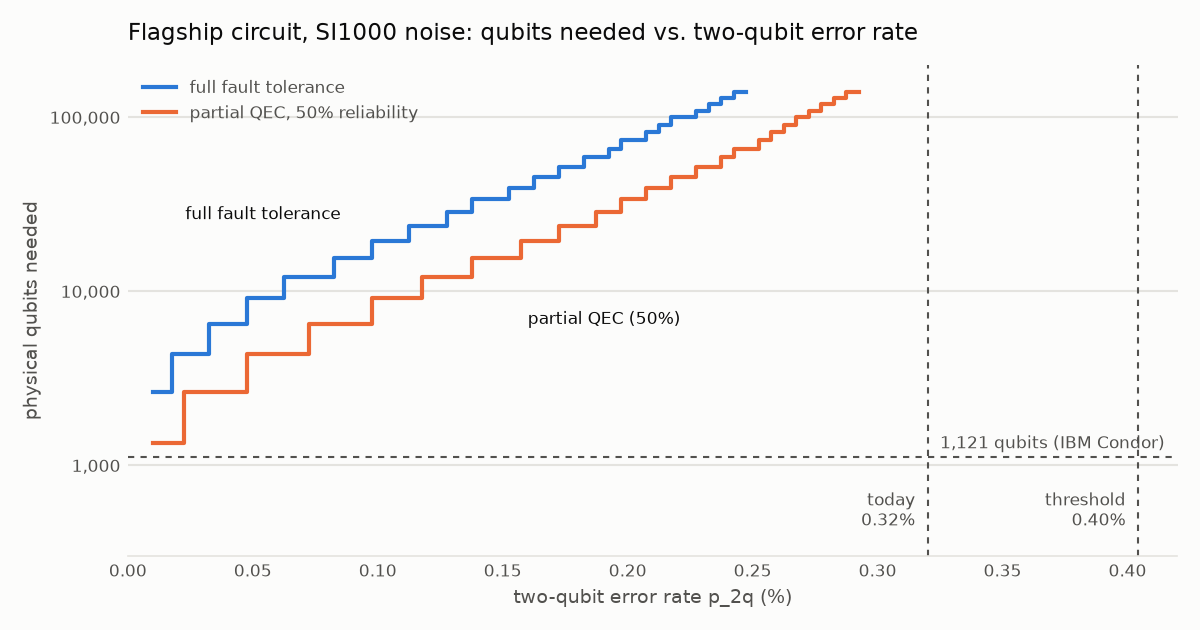
\includegraphics[width=\linewidth]{figs/error_rate_sweep.png}
\caption{Physical qubits needed by \texttt{shor\_like\_sequential.qasm}
under SI1000 noise, as a function of the two-qubit error rate. At today's
$0.32\%$ neither full fault tolerance nor partial QEC exists for any $d\leq51$.}
\label{fig:error-rate-sweep}
\end{figure}

\paragraph{Reframing the question: not pass/fail, but which confidence quartile is actually reachable.}
A hard budget need not produce a binary answer. We added a second query
(\texttt{best\_feasible\_within\_hard\_budget()}) that asks a different,
arguably more honest question: given that the budget $B$ is fixed and
non-negotiable, what is the \emph{best} reliability reachable at all
(the largest $d$ whose cost still fits $B$, regardless of whether it
clears any target), and which confidence quartile does that reliability
fall into --- $[0,25\%)$ low, $[25,50\%)$ low-moderate, $[50,75\%)$
moderate, $[75,100\%]$ high? Sweeping the budget itself for this same
circuit on the trapped-ion H2 profile makes the shape of the tradeoff concrete:

\begin{table}[t]
\centering\footnotesize
\begin{tabular}{rrrl}
\toprule
Budget $B$ & Best $d$ & Reliability & Quartile \\
\midrule
1{,}121 (declared) & 3 & $\sim$0\% & low \\
2{,}000 & 5 & 1.3\% & low \\
3{,}000 & 7 & 59.7\% & moderate \\
5{,}000 & 9 & 94.1\% & high \\
7{,}000 & 11 & 99.3\% & high \\
\bottomrule
\end{tabular}
\caption{Best reliability actually reachable at a hard qubit budget
(\texttt{shor\_like\_sequential.qasm}, trapped-ion H2, $p_{2q}=0.1\%$), reported by confidence quartile
rather than as pass/fail against a single target.}
\label{tab:budget-quartile}
\end{table}

At the project's declared $1{,}121$-qubit budget, the honest answer is
not ``no code helps'' in the abstract --- it is that even the cheapest
real surface-code patch ($d=3$, $486$ qubits) already uses $43\%$ of the
budget while delivering essentially no protection (reliability
$\sim 10^{-16}$, lowest quartile): the budget is simply too small
relative to this circuit's T-count for \emph{any} distance to matter yet.
Reliability only leaves the lowest quartile once the budget reaches
roughly $2.4\times$ the declared one ($\approx2{,}650$ qubits, $d=7$), where it
jumps straight to the moderate quartile. This is a more useful statement
than a single pass/fail bit: it tells a reader exactly how much budget
growth would be needed before partial QEC becomes worth considering for
this circuit, instead of leaving ``the budget is insufficient'' as an
unquantified dead end.

\subsection{Proposition 3: monotonicity of the calibrated cost/reliability trade-off, and correctness of the sweep}
\label{sec:prop3}
Sections~\ref{sec:decision-formal} and~\ref{sec:partial-qec} both rely, as
a design choice stated only in code comments, on two claims that were
never actually proved: that cost grows monotonically with distance $d$
(so a single ascending scan over $d$, stopping at the first budget-exceeding
value, is safe), and that reliability grows monotonically with $d$ (so the
largest affordable $d$ is automatically the most reliable affordable
choice, and the confidence-quartile staircase of
Table~\ref{tab:budget-quartile} cannot move backwards as the budget grows).
Both claims turn out to be provable directly from the two closed-form
functions this project already validated and uses --- no new theorem from
the literature is needed, only algebra applied honestly to formulas we
already committed to.

\begin{proposition}
Fix $n\geq 1$ logical qubits, tcount $t\geq 1$, and physical error rate
$0<p<p_{\mathrm{th}}$ (the fitted threshold of
Section~\ref{sec:tools-open-estimator}). Using this project's own
surface-code physical-qubit formula
$N_{\mathrm{data}}(d)=2d^2$ (Litinski's tile; Section~\ref{sec:tools-open-estimator}) and the Litinski~\cite{litinski2019game}
15-to-1 factory formula $N_{\mathrm{fac}}(d)=22d^2$ (one factory), define
$\mathrm{Cost}(d) = n\cdot N_{\mathrm{data}}(d) + N_{\mathrm{fac}}(d)$ and,
using this project's own calibrated fit for any one noise model
$p_L(d)=A\cdot(p/p_{\mathrm{th}})^{(d+1)/2}$,
$\mathrm{Reliability}(d) = (1-p_L(d))^{nt}$. Then, on the odd-integer domain
$d\in\{3,5,7,\ldots\}$ where $p_L(d)\in[0,1)$:
\begin{enumerate}
\item[(a)] $\mathrm{Cost}(d)$ is strictly increasing in $d$.
\item[(b)] $\mathrm{Reliability}(d)$ is strictly increasing in $d$.
\end{enumerate}
\end{proposition}

\begin{proof}
(a) $\mathrm{Cost}(d) = (2n+22)d^2$ with $2n+22>0$ (since $n\geq1$), which
is strictly increasing for every $d>0$, with no dependence on $n$, $t$, or $p$.

(b) Write $r=p/p_{\mathrm{th}}\in(0,1)$ (guaranteed by $p<p_{\mathrm{th}}$).
The exponent $(d+1)/2$ is strictly increasing in $d$, and $x\mapsto r^x$ is
strictly decreasing on $x\in\mathbb{R}$ whenever $r\in(0,1)$; composing a
strictly increasing exponent with a strictly decreasing base-$r$ power
gives $p_L(d)=A\cdot r^{(d+1)/2}$ strictly decreasing in $d$ (for the fixed
constant $A>0$ from the fit). Hence $1-p_L(d)$ is strictly increasing in
$d$, and on the domain where $1-p_L(d)\in(0,1]$, the map
$x\mapsto x^{nt}$ is strictly increasing for any fixed $nt\geq 1$; composing
gives $\mathrm{Reliability}(d)=(1-p_L(d))^{nt}$ strictly increasing in $d$.
\end{proof}

\begin{corollary}
Two consequences, both previously assumed in code but not proved:
\begin{itemize}
\item \emph{Correctness of the ascending sweep.} By (a), the first
$d$ found while scanning upward is automatically the cheapest $d$; by
(b), the largest $d$ whose cost still fits a hard budget $B$ is
automatically the most reliable option affordable under $B$. Both
\texttt{sweep\_partial\_qec()} and
\texttt{best\_feasible\_within\_hard\_budget()} can therefore stop at the
first threshold crossing rather than exhaustively searching all $d$ up to
$d_{\max}$: this is a proved optimality guarantee, not merely an
efficiency shortcut.
\item \emph{The budget-quartile staircase cannot regress.} Since the
best-affordable $d$ is non-decreasing in the budget $B$ (larger $B$ can
only admit larger-or-equal $d$, never fewer options) and
$\mathrm{Reliability}(d)$ is strictly increasing in $d$ by (b), the
best-achievable reliability reported by
\texttt{best\_feasible\_within\_hard\_budget(B)} is non-decreasing in
$B$. Table~\ref{tab:budget-quartile}'s quartile column is therefore
guaranteed, by construction of the calibrated model, never to drop to a
lower confidence quartile as $B$ increases --- the observed staircase is
a structural property of the model, not a coincidence of the six budget
values we happened to sweep.
\end{itemize}
\end{corollary}

\paragraph{Scope, stated honestly.} This proposition proves internal
consistency of the calibrated model and the algorithms built on it --- it
does \emph{not} validate the model itself at small $d$, which
Section~\ref{sec:partial-qec} already flags as extrapolated below the
calibrated range ($d\geq5$). A model that is wrong at $d=3$ would
still satisfy this proposition (monotonicity is a property of the fitted
functional form $A\cdot r^{(d+1)/2}$ for any fit constants $A,p_{\mathrm{th}}$,
not evidence that those constants are accurate that low); the two
questions --- ``is the sweep algorithm correct given the model'' and ``is
the model itself accurate at small $d$'' --- are independent, and this
proposition only answers the first.

\FloatBarrier
\section{Stress test: scale, learned predictors, and operational cost}
\label{sec:stresstest}
Every result so far was measured on this project's original 98-instance,
9-family dataset (circuits up to 20 qubits) or on the 9 hand-picked
reference circuits. Four questions were left open by that scope: does the
deployed rule generalize to circuits genuinely larger than any it was
calibrated on; does combining features with standard machine learning beat
the single-feature rule when evaluated with the same LOFO honesty already
used elsewhere; how expensive is running this pipeline in practice; and what
do the answers mean for planning around evolving hardware. This section
answers all four with new experiments, not new claims.

\subsection{Generalization to circuits larger than the calibration set}
\label{sec:stresstest-scale}
We generated 21 new circuit instances, never seen by any rule or model in
this project, reusing the exact same family generators as the original
98-instance dataset (\texttt{build\_circuit\_dataset.py},
\texttt{build\_circuit\_dataset\_v2.py}) but at sizes larger than any
instance previously used --- up to 32 qubits (GHZ), versus a previous
maximum of 20. Three QFT instances ($n{=}16,20,24$) initially failed at the
QASM export step with a numeric-precision bug (a phase value formatted too
small to re-parse, \texttt{TypeError: Phase expression `\ldots' contains
unbound variables}); this and two further bugs this stress test surfaced
were fixed during the same session (Section~\ref{sec:stresstest-bugfixes}
gives the full before/after). Ground-truth ZX-calculus gain was measured
on all 21/21 circuits post-fix; the deployed-rule \emph{accuracy} check
below additionally excludes \texttt{QFT\_n20}/\texttt{n24} for an
unrelated, separate reason found while fixing these bugs --- pyzx's own
QASM parser (independent of anything this project's code does) scales
very poorly with the number of \emph{distinct phase literals}, and QFT has
$O(n^2)$ of them; Section~\ref{sec:stresstest-bugfixes} documents this as
a declared, out-of-scope, third-party limitation rather than a fourth
in-scope bug. The accuracy check below therefore covers 19 instances
across 9 families.

\begin{table}[t]
\centering\footnotesize
\begin{tabular}{lrr}
\toprule
& Original dataset & Held-out large set \\
\midrule
Max.\ qubits & 20 & 32 \\
Deployed rule accuracy & 70.4\% (LOFO) & 73.7\% \\
Majority baseline & --- & 57.9\% \\
\bottomrule
\end{tabular}
\caption{The already-deployed \texttt{zx\_calculus} rule, evaluated on 19
circuit instances larger than any used to calibrate it, beats the
majority-class baseline in this set by 15.8 points --- unlike its
in-distribution LOFO result, which does not beat baseline.}
\label{tab:largescale}
\end{table}

The rule's two real failure modes on this set are informative rather than
uniform noise: it missed all four large QAOA instances ($n{=}20,24$,
density $0.3$ and $0.6$) --- the diagonal-cost-layer motif detector
(Section~\ref{sec:qasm-tool}) that correctly flagged 24/24 QAOA instances
in the original dataset did not fire on these larger, sparser ones, a
genuine generalization gap in that specific detector; and it missed one
random-circuit instance (\texttt{Random\_n24\_depth16}) where ZX-calculus
actually \emph{increased} T-count ($-3.8\%$ ``gain''), a case the rule has
no mechanism to anticipate at all. Both are reported as open, unresolved
gaps, not smoothed over.

\subsection{Does combining features with machine learning help, honestly evaluated?}
\label{sec:stresstest-ml}
An earlier iteration of this project trained a decision tree (85.1\%) and a
logistic regression (88.8\%) combining several structural features, but
with ordinary 5-fold cross-validation on a smaller 62-instance dataset ---
not leave-one-family-out (LOFO). That combined-feature approach was never
re-evaluated with the same LOFO honesty already applied to the
single-feature rule (which fell from a reported 82.9\% to 70.4\%, a
retraction discussed in Section~\ref{sec:results}). We did so here: both
models, now given every structural feature this project has computed for
the full 98-instance dataset (including tensor-network contraction cost,
previously used only as a 9-point correlation, here as a real per-instance
feature), evaluated with genuine \texttt{LeaveOneGroupOut} cross-validation
by family.

\begin{table}[t]
\centering\footnotesize
\begin{tabular}{lrr}
\toprule
Evaluation & Log.\ regression & Decision tree \\
\midrule
LOFO (9 families, pooled) & 62.2\% & 52.0\% \\
Large-scale held-out (\S\ref{sec:stresstest-scale}) & 94.7\% & 94.7\% \\
\bottomrule
\end{tabular}
\caption{Same models, two different notions of generalization. Majority
baseline is 66.3\%; the deployed single-feature rule scores 70.4\% (LOFO)
and 73.7\% (large-scale).}
\label{tab:mlgen}
\end{table}

The honest result is a real negative extended, plus a genuine nuance.
\textbf{Negative, confirmed:} combining more features with standard ML,
evaluated on circuit families the model has never seen, does \emph{not}
beat the majority baseline (62.2\% and 52.0\%, both below 66.3\%) --- the
existing single-feature rule's 70.4\% remains, honestly, the best
family-generalizing predictor found across this entire project.
\textbf{Nuance, new:} the same two models, trained once on all 98
instances and evaluated on the 19 large circuits of
Section~\ref{sec:stresstest-scale} (new \emph{instances}, but of families
the model \emph{has} seen, just at a scale it has not), reach 94.7\% ---
clearly beating both the majority baseline and the deployed rule's 73.7\%
in that same set. These are different generalization questions: ML here
fails to generalize to a genuinely new circuit \emph{family}, but
generalizes well to a new \emph{scale} of a familiar one. Reporting both
numbers, rather than only the flattering one, is the point.

\subsection{Operational cost of the decision layer itself}
\label{sec:stresstest-latency}
A decision layer that recommends a regime is only useful if computing that
recommendation is itself cheap enough to run before dispatching a job. We
timed the real, deployed pipeline (\texttt{profile\_circuit} +
\texttt{recommend\_techniques}) end to end. The numbers below are
\emph{after} the fixes of Section~\ref{sec:stresstest-bugfixes}; that
section gives the original, broken numbers this stress test first found.

\begin{table}[t]
\centering\footnotesize
\begin{tabular}{lrr}
\toprule
Circuit & Qubits & Wall time \\
\midrule
\texttt{vqe\_ansatz.qasm} & 8 & 0.06 s \\
\texttt{qft10.qasm} & 10 & 0.18 s \\
\texttt{qaoa\_farm.qasm} & 17 & 0.41 s \\
\texttt{adder8.qasm} & 18 & 0.99 s \\
\texttt{shor\_like\_sequential.qasm} (flagship) & 16 & 11.6 s \\
\bottomrule
\end{tabular}
\caption{End-to-end wall time, \texttt{profile\_circuit} +
\texttt{recommend\_techniques(profile=\ldots)}, on the project's own
reference circuits, post-fix.}
\label{tab:latency}
\end{table}

All five reference circuits are now practical to run before dispatch,
including the flagship (11.6 s, down from 44.4 s pre-fix --- see
Section~\ref{sec:stresstest-bugfixes}). The remaining cost on the flagship
is pyzx's own QASM-parsing step (a third-party, `lark`-grammar-based
parser invoked once per gate for phase expressions), not anything this
project's code still does redundantly. The honest remaining limit,
documented in the next section: pyzx's parser itself scales poorly with
the number of \emph{distinct phase literals} in a circuit (not qubit
count), which is now the dominant, out-of-scope bottleneck for
phase-heavy circuits like large QFT instances.

\subsection{Bugs found and fixed}
\label{sec:stresstest-bugfixes}
This stress test surfaced three concrete, in-scope bugs in this project's
own code (not in any external library), all found by trying to run the
pipeline at a scale it had never been run at before, and all fixed in the
same session rather than left as declared limitations.

\textbf{Bug 1: duplicated \texttt{profile\_circuit()} calls.} The common
call pattern used throughout this project's own scripts,
\texttt{p = profile\_circuit(path)} followed by
\texttt{recs = recommend\_techniques(path)}, silently computed the
\emph{entire} circuit profile twice, because \texttt{recommend\_techniques()}
always recomputed it internally regardless of whether the caller already
had it. \emph{Fix:} \texttt{recommend\_techniques()} now takes an optional
\texttt{profile=} argument and skips recomputation when given one; the one
caller in this project that had the duplicated pattern
(\texttt{qasm\_tool.analyze\_circuit}) was updated to pass it through.
\emph{Effect, measured on the flagship circuit:} 44.4~s~$\to$~11.6~s
(35.2~s of which was the second, now-eliminated, parse-plus-QCP-tracking
pass).

\textbf{Bug 2: exponential memory allocation in the QCP tracker.} This is
the one that actually caused the $>$60~s hangs. In
\texttt{qcp\_bounded\_tracker.py}, every merged qubit group --- including
one about to be marked \texttt{known=False} (``abandon tracking'', the
exact mechanism meant to keep this bounded) --- unconditionally allocated
a dense state vector of size $2^{|\text{qubits in group}|}$ in its
constructor, before checking whether it would ever be used. A circuit with
real entanglement merges such groups repeatedly; by 22--24 qubits this
routinely tried to allocate hundreds of megabytes to gigabytes for a
vector that was about to be discarded unread. \emph{Fix:} the constructor
now takes a \texttt{known} flag and skips the allocation entirely when
\texttt{False}, since no code path reads \texttt{.state} for an unknown
group. \emph{Effect, measured directly on the circuit that hung}
(\texttt{Adder\_n10}, 22 qubits): $>$60~s (killed) $\to$ 0.18~s.

\textbf{Bug 3: unparseable scientific notation in exported QASM.}
\texttt{qiskit.qasm2.dumps()} writes very small rotation angles in
scientific notation (e.g.\ \texttt{9.587...e-05}); pyzx's QASM parser
cannot parse that notation at all and fails with a misleading
\texttt{unbound variables} error, as if the number were a symbolic
variable. Verified directly: the identical value written in plain decimal
notation parses without issue. \emph{Fix:} a small utility
(\texttt{qasm\_safe\_export.py}) that rewrites any scientific-notation
literal in QASM text to its plain-decimal equivalent before handing it to
pyzx, applied at the two circuit-generation scripts that build large
circuits for this stress test. \emph{Effect:} the three previously-failing
QFT instances ($n{=}16,20,24$) now parse and measure correctly; ground
truth is now available for 21/21 circuits in
Section~\ref{sec:stresstest-scale} (up from 18/21).

\textbf{A fourth issue found while fixing the above, addressed but
distinct from the three bugs:} once Bug 2 stopped masking it, a separate
cost became visible --- the exact-statevector entanglement probe
(\S\ref{sec:entanglement-metric}) is expensive near its own declared
24-qubit cap for some circuits (e.g.\ \texttt{GHZ\_n24}, only 24 gates,
still took $>$40~s), evidently memory- rather than gate-count-bound. We
lowered \texttt{\_MAX\_QUBITS\_FOR\_EXACT\_ENTANGLEMENT\_PROBE} from 24 to
20, the largest size confirmed fast in practice, rather than leave a
``practical, not theoretical'' cap that in practice still hung the
pipeline before reaching its own graceful-degradation path.

\textbf{Bug 4, found after release: the logical error budget counted one
patch, not $n$.} The fitted $p_L(d)$ is a per-patch rate over $d$ rounds
(a rotated-memory experiment with $d$ rounds), and each T-gate takes about
$d$ rounds, during which \emph{every} logical patch can fail. The FTQC
estimator nonetheless split the error budget over tcount events instead of
$n\cdot$tcount, and the partial-QEC sweep used $(1-p_L)^{\text{tcount}}$
instead of $(1-p_L)^{n\cdot\text{tcount}}$. For the flagship circuit
($n=16$) the design point $d=23$ actually carried a total logical error
of $\approx9.4\%$, not the declared $\le1\%$. \emph{Fix:} both now use
$n\cdot$tcount. \emph{Effect} (under the single $0.74\%$ fit then in use): full FTQC rises from $29{,}654$ to
$46{,}790$ physical qubits ($d=23\to29$), partial QEC reaches the $0.5$
target at $d=19$ and $20{,}390$ qubits instead of $d=13$ and $9{,}734$, and
the partial-QEC saving shrinks from $\sim\!3\times$ to $\sim\!2.3\times$.
The qualitative verdict for the flagship circuit (an unresolved gap at the
declared budget) was unchanged.

\textbf{Bug 5, found by cross-checking with Deltakit: the qubit count and
the noise model.} Two further problems surfaced when we rebuilt the
surface-code memory experiments with an independent toolchain
(Section~\ref{sec:tools-open-estimator}, \texttt{examples/deltakit\_crosscheck.py}).
(i) The per-logical-qubit count $2d^2+3d-1$ was \texttt{stim.Circuit.num\_qubits},
which counts unused qubit indices of Stim's generator; a rotated patch uses
$2d^2-1$. We now use $2d^2$ (Litinski's tile, routing included). (ii) The
single $0.74\%$ threshold came from a noise model with no idle errors and
cheap measurement; per-noise-model fits give $0.40\%$ (SI1000,
superconducting) and $0.85\%$ (ToyNoise, trapped ion). \emph{Effect:} (ii)
dominates. On the superconducting profile the flagship circuit goes from
``FTQC at $46{,}790$ qubits'' to ``no distance up to 51 works'', so the
flagship results of Section~\ref{sec:partial-qec} are now reported on the
trapped-ion H2 profile (FTQC $6{,}534$ qubits, partial QEC $2{,}646$), with
the superconducting case reported as the error rate it must reach first.
Every number in this paper uses the corrected model.

\textbf{What remains open, honestly:} pyzx's own QASM parser is slow for
circuits with many \emph{distinct} phase literals (demonstrated:
\texttt{QFT\_n16} 2.3~s, \texttt{QFT\_n20} 25.2~s, \texttt{QFT\_n24} did
not complete in several minutes) --- a third-party performance
characteristic, not a bug in this project's code, and out of scope to
patch here. The large-scale accuracy check of
Section~\ref{sec:stresstest-scale} therefore excludes
\texttt{QFT\_n20}/\texttt{n24} specifically (19 of 21 circuits), while
still reporting their ground-truth ZX-calculus gain, which needed no full
pipeline run to measure.

\subsection{What this means for planning around evolving hardware}
\label{sec:stresstest-practical}
Putting Sections~\ref{sec:stresstest-scale}--\ref{sec:stresstest-latency}
together with the crossover sweep of Section~\ref{sec:crossover} and the
budget-quartile table of Section~\ref{sec:partial-qec} gives a more
concrete answer than either alone to ``what should a team actually do as
hardware grows'': (i) the regime decision is not fixed once --- as the
declared qubit budget grows along the trajectory implied by
Table~\ref{tab:budget-quartile} ($1{,}121\to15{,}000$), the same flagship
circuit moves from the lowest confidence quartile to \emph{high}
confidence without changing anything about the circuit itself, so a
hardware roadmap and a circuit-reduction roadmap answer the same question
from two directions and should be planned together, not separately; (ii)
because Proposition~3 (\S\ref{sec:prop3}) proves this progression cannot
reverse, a team can commit to re-running the sweep as budget grows and
trust that reliability only improves, without re-deriving that guarantee
each time; (iii) because the deployed technique-recommendation rule
degrades gracefully rather than catastrophically at larger scale (still
15.8 points above baseline out-of-distribution, Table~\ref{tab:largescale}),
it remains a reasonable default to consult automatically before dispatch
even as circuits grow past this project's calibration range, provided its
two known failure modes (large sparse QAOA-like circuits, and rare
negative-gain instances) are flagged for manual review rather than trusted
blindly; and (iv) the operational-cost finding of
Section~\ref{sec:stresstest-latency} identified a concrete near-term
engineering priority --- removing the duplicate \texttt{profile\_circuit()}
call and bounding the QCP-tracking sub-step's cost --- ahead of any further
accuracy work, since a predictor that cannot run in real time before
dispatch is not operationally useful regardless of its accuracy; both were
fixed within the same session (Section~\ref{sec:stresstest-bugfixes}), cutting
flagship-circuit latency by 74\% (44.4~s~$\to$~11.6~s) and eliminating the
$>$60~s hangs entirely, leaving pyzx's own third-party QASM-parsing cost
for phase-heavy circuits as the one remaining, out-of-scope bottleneck.

\FloatBarrier
\section{Discussion: strengths and limitations by scenario}
Rather than a single verdict, different parts of this system have different,
separately measured confidence levels. \textbf{High confidence}: the exact
T-count-fraction-zero filter for ZX-calculus; Azure QRE-based FTQC resource
estimates (a mature, externally validated tool); the surface-code threshold
measurement (consistent with theory). \textbf{Moderate, honestly bounded
confidence}: the $70.4\%$ default ZX-calculus recommendation, now reported
without inflation. \textbf{Open, declared limitations}: QAOA-type circuits
remain unclassifiable by any tested feature; the SabreSwap density anomaly
at density $1.0$ is unexplained; the RQAOA-style rounds metric has no
external benchmark; and the tensor-network/ZX-gain correlation
($r=0.66$) is suggestive but statistically underpowered ($n=9$).

\section{Reproducibility}
\label{sec:reproducibility}
All code, datasets, and figures in this paper are packaged in an
accompanying public repository organized as an open validation guide (in
the spirit of Unitary Foundation's Metriq, but populated with this
project's own executed experiments): per-technique folders with code and a
scope/limitations README, a real QEC folder, the decision-layer code, a
benchmarks folder with the corrected predictor table, and a papers folder
mapping every external claim to what it confirms. A discrepancy between an
original run and an independent re-run of the SabreSwap density sweep
(different random graph instance, same qualitative anomaly, different
absolute magnitude) is documented rather than silently resolved.

\section{Conclusion}
Circuit-reduction technique selection measurably changes the QEM-vs-FTQC
decision, and every technique tested here has a real, narrow, and now
precisely measured domain of applicability rather than a universal verdict.
The most important methodological result of this paper is not a single
number but a discipline: two independent findings that looked like genuine
discoveries (a phase-polynomial reimplementation, and an $82.9\%$ predictor)
were rejected or corrected only because they were checked against a harder
standard (unitary equivalence; full-dataset LOFO) before being reported as
real. We believe that discipline, more than any individual result, is what
should travel with this project into its next phase.

\paragraph{From calibrated rules to provable claims.} Section~\ref{sec:new-theory}
took that same discipline one step further: rather than stop at a
calibrated empirical rule, we asked whether it could be proved, and were
honest about the answer differing by case. Proposition~1
(Section~\ref{sec:prop1}) upgrades the ZX-calculus diagonal-layer blind
spot from an observed $0\%$-reduction pattern to a proved structural fact,
with a short, checkable proof grounded in phase-polynomial theory and
Boolean Fourier analysis already adjacent to this project's tools.
Proposition~2 (Section~\ref{sec:prop2}) shows the limit of that ambition
just as clearly: treewidth of a circuit's static topology is a real,
provable, necessary condition (Markov \& Shi~\cite{markovshi2008}) for a
classical tensor-network shortcut, but we found, by actually running the
certificate, that it is not sufficient for our own flagship circuit's
depth regime --- a favorable topological score (treewidth $1$ for the
heavy-hex-derived circuit) coexists with the highest measured entanglement
fraction ($59.5\%$) of any reference circuit, a genuine and unexpected
result of combining the two metrics rather than trusting either alone.
Section~\ref{sec:decision-formal} then closed the loop on the paper's
core question by \emph{formalizing} (not proving --- we are careful to
keep this distinction) the QEM-vs-FTQC choice itself as a constrained
optimization problem built from these validated pieces. Run honestly over
the reference set, it mostly returns a declared null result (FTQC never
fits the budget at this scale, so QEM wins by default), but for
\texttt{shor\_like\_sequential.qasm} --- again our own flagship, again the
circuit Propositions~1--2 could not clear --- it reports an explicit,
quantified gap that neither QEM nor FTQC closes, which is exactly the
space a partial QEC scheme would need to fill. Section~\ref{sec:partial-qec}
took a first, honestly-bounded step at that estimate --- sweeping the
same validated surface-code model to smaller distances rather than only
solving for full fault tolerance --- and found a real, quantified
$\sim\!2.5\times$ reduction in qubit cost for the same reliability bar on
trapped-ion hardware ($2{,}646$ vs.\ $6{,}534$ qubits), not yet enough to
close this particular gap within the declared budget, but a genuine partial
answer in a space this project previously could only point at. On
superconducting hardware under realistic SI1000 noise the answer is
starker: at $0.32\%$ no surface-code distance helps this circuit, and the
useful output is the error rate the hardware must reach first ($\approx0.25$--$0.29\%$
for any correction to work, $\approx0.1\%$ for it to be affordable). Proposition~3
(Section~\ref{sec:prop3}) then closed a smaller but real rigor gap in
that same machinery: the monotonicity of cost and reliability in $d$,
used throughout Sections~\ref{sec:decision-formal}--\ref{sec:partial-qec}
as an unproved code-level assumption, is in fact a short, direct
consequence of the two closed-form formulas this project already
validated --- turning ``the sweep algorithm happens to work'' into ``the
sweep algorithm is provably correct given the calibrated model,'' while
being explicit that this says nothing new about whether the calibrated
model itself is accurate at the small distances the sweep explores.

\paragraph{Stress-testing generality, honestly --- and fixing what it broke.}
Section~\ref{sec:stresstest} took the project's biggest untested
assumption --- that results calibrated on $\leq\!20$-qubit circuits and a
fixed feature set generalize --- and tested it directly rather than
asserting it. The deployed rule holds up better than expected at larger
scale (73.7\% vs.\ a 57.9\% baseline on 19 new, larger, never-seen
circuits); standard machine learning, evaluated with the same LOFO honesty
as everywhere else in this paper, does \emph{not} beat that simple rule
when generalizing to an unseen circuit \emph{family} (62.2\%, below
baseline) but generalizes very well to unseen \emph{scale} within a
familiar family (94.7\%) --- a genuine, useful distinction this project
had not previously drawn. That same stress test also found three real bugs
in this project's own code (a duplicated expensive call, an exponential
memory allocation hidden behind a size cap that didn't bound it, and an
unparseable QASM edge case) --- all three fixed within the session
(Section~\ref{sec:stresstest-bugfixes}), cutting the flagship circuit's
latency by 74\% (44.4~s~$\to$~11.6~s) and turning $>$60~s hangs at 22
qubits into sub-second results. What remains open is now precisely scoped
and attributed correctly: a third-party parsing bottleneck in pyzx itself,
not in this project's code.

\paragraph{What the comparison against a landmark result adds.} Testing
this pipeline against a real, external, peer-reviewed benchmark --- Kim et
al.'s 2023 Nature ``quantum utility'' experiment, rather than only our own
synthetic circuit families --- changes what we can honestly claim, in five
concrete ways:
\begin{enumerate}
  \item \textbf{The hardware-agnostic, QASM-in architecture holds up
  against a real circuit family we did not design.} A 16-qubit subgraph
  extracted directly from a real device's coupling map (\texttt{FakeTorino}),
  not hand-drawn, ran through the same unmodified \texttt{qasm\_tool.py}
  used for our synthetic circuits, across all three hardware profiles,
  with no circuit-specific code.
  \item \textbf{The same real circuit family exposed and fixed a genuine
  false negative} in \texttt{recommend\_techniques()} (the degree-gated
  \texttt{qaoa\_like\_pattern} condition), because
  our synthetic test set never included a sparse (max-degree-3), diagonal-cost
  circuit --- the fix (Section~\ref{sec:qasm-tool}) generalizes the
  detector beyond dense QAOA-style graphs to any single diagonal
  Hamiltonian layer.
  \item \textbf{Our own FTQC cost estimate on this circuit
  ($12{,}854$ physical qubits) quantifies exactly why IBM ran it as a
  NISQ+QEM experiment rather than waiting for fault tolerance} --- the
  QEM-vs-FTQC decision this whole project is built around is not
  hypothetical for this circuit, it is the decision IBM actually made.
  \item \textbf{The ZNE mechanism itself is reproducible and quantifiable
  at a scale we can fully verify against exact simulation}, not just
  citable from the paper: a genuine null result at shallow depth (noise
  bias below the shot-noise floor) and a genuine $\sim$42\% error
  reduction at depth matched to the paper's own scale.
  \item \textbf{The Tindall et al.\ rebuttal is the most consequential
  finding of this comparison}: it shows that circuit size and measured
  entanglement alone do not establish classical intractability, and that
  this blind spot is shared by every resource estimator tested in this
  project, including our own. We treat this not as a reason to discount
  the comparison but as its main deliverable --- it motivated a new,
  routine, low-confidence entanglement-fraction metric
  (Section~\ref{sec:entanglement-metric}) now wired into the pipeline,
  and that metric's most important output was a complication about our
  own flagship circuit, reported honestly rather than omitted.
\end{enumerate}

\bibliographystyle{plain}
\begin{thebibliography}{9}
\footnotesize
\bibitem{kissinger2019} A.~Kissinger, J.~van~de~Wetering, ``Reducing T-count
with the ZX-calculus,'' arXiv:1903.10477 (2019).
\bibitem{amy2014} M.~Amy, D.~Maslov, M.~Mosca, ``Polynomial-Time T-Depth
Optimization of Clifford+T Circuits via Matroid Partitioning,'' IEEE TCAD
33(10), 2014.
\bibitem{bravyi2020} S.~Bravyi et al., ``Obstacles to Variational Quantum
Optimization from Symmetry Protection,'' PRL 125, 260505 (2020) (RQAOA).
\bibitem{fowler2012} A.~Fowler, M.~Mariantoni, J.~Martinis, A.~Cleland,
``Surface codes: Towards practical large-scale quantum computation,'' Phys.
Rev.\ A 86, 032324 (2012).
\bibitem{boixo2018} S.~Boixo et al., ``Characterizing quantum supremacy in
near-term devices,'' Nature Physics 14, 595--600 (2018).
\bibitem{spielman2011} D.~Spielman, N.~Srivastava, ``Graph Sparsification by
Effective Resistances,'' SIAM J.\ Comput.\ 40(6), 2011.
\bibitem{azureqre} Microsoft, ``Azure Quantum Resource Estimator''
documentation, \url{https://learn.microsoft.com/azure/quantum/}.
\bibitem{qiskitcutting} Qiskit Addon Cutting documentation,
\url{https://qiskit.github.io/qiskit-addon-cutting/}.
\bibitem{metriq} Unitary Foundation, ``Metriq: Community-driven quantum
benchmarks,'' \url{https://metriq.info/}.
\bibitem{perlin2026} M.~A.~Perlin, Z.~He, A.~Alexiades~Armenakas,
P.~Andres-Martinez, T.~Hao, D.~Herman, Y.~Jin, K.~Mayer, C.~Self,
D.~Amaro, C.~Ryan-Anderson, R.~Shaydulin, ``Fault-tolerant execution of
error-corrected quantum algorithms,'' arXiv:2603.04584 (2026).

\bibitem{qgss2025lab2} J.~Mart\'inez de Lejarza, A.~Maldonado (advised by
M.~Pfaffhauser, P.~Nation, J.~Huang, S.~Shin), ``Lab 2: Noise, Transpilation
and Error Mitigation,'' IBM Qiskit Global Summer School 2025,
\url{https://github.com/qiskit-community/qgss-2025/blob/main/solutions/lab-2/lab2-solution.ipynb}
(2025).

\bibitem{kissinger2019reducing} A.~Kissinger, J.~van de Wetering,
``Reducing T-count with the ZX-calculus,'' Physical Review A 102, 022406
(2020), arXiv:1903.10477.

\bibitem{spacetimeopt2025} ``Space-Time Optimisations'' for lattice-surgery
compilation, arXiv:2511.08848 (2025).

\bibitem{latticesurgerycompiler2025} ``A Resource Allocating Compiler for
Lattice Surgery,'' arXiv:2506.04620 (2025).

\bibitem{litinski2019game} D.~Litinski, ``A Game of Surface Codes:
Large-Scale Quantum Computing with Lattice Surgery,'' Quantum 3, 128
(2019), arXiv:1808.02892.

\bibitem{quantinuum2026iceberg} Quantinuum, real-hardware demonstration of
error-detected and concatenated iceberg-code logical qubits on the Helios
processor (up to 94 error-detected / 48 error-corrected logical qubits,
$[[80,48,4]]$ code), reported March 2026; this postdates our training data
and is cited from contemporaneous web coverage, not verified against the
original preprint: \url{https://thequantuminsider.com/2026/03/10/quantinuum-researchers-demonstrates-quantum-computations-with-dozens-of-protected-logical-qubits/}
and \url{https://postquantum.com/quantum-research/quantinuum-94-logical-qubits/}.

\bibitem{ibmcondor2023} IBM, ``Condor'' 1{,}121-superconducting-qubit
processor, announced December 2023 -- cited here only as an order-of-magnitude
reference for the largest total physical qubit count publicly reported for a
single real device, not as a claim about its logical-qubit capability.

\bibitem{kim2023utility} Y.~Kim, A.~Eddins, S.~Anand, K.~X.~Wei,
E.~van~den~Berg, S.~Rosenblatt, H.~Nayfeh, Y.~Wu, M.~Zaletel, K.~Temme,
A.~Kandala, ``Evidence for the utility of quantum computing before fault
tolerance,'' Nature 618, 500--505 (2023).

\bibitem{tindall2023tensor} J.~Tindall, M.~Fishman, E.~M.~Stoudenmire,
D.~Sels, ``Efficient tensor network simulation of IBM's Eagle kicked
Ising experiment,'' PRX Quantum 5, 010308 (2024), arXiv:2306.14887.
\bibitem{markovshi2008} I.~L.~Markov, Y.~Shi, ``Simulating Quantum
Computation by Contracting Tensor Networks,'' SIAM J.\ Comput.\ 38(3),
963--981 (2008), arXiv:quant-ph/0511069.
\bibitem{griffithsniu1996} R.~B.~Griffiths, C.-S.~Niu, ``Semiclassical
Fourier Transform for Quantum Computation,'' Phys.\ Rev.\ Lett.\ 76,
3228 (1996), arXiv:quant-ph/9511007.
\bibitem{farhi2014} E.~Farhi, J.~Goldstone, S.~Gutmann, ``A Quantum
Approximate Optimization Algorithm,'' arXiv:1411.4028 (2014).
\end{thebibliography}

\end{document}
